% !TeX spellcheck = en_US
\documentclass[11pt, a4paper, english, hidelinks, twoside, openright]{report}
% Fixes the "no room for \count error"
% @see http://tex.stackexchange.com/questions/186588/what-does-the-etex-package-do-exactly
\usepackage{etex}
\usepackage{babel}
% All pages with no text (generated in order to have chapters start on odd numbered pages) will be completely empty.
\usepackage{emptypage}	
\usepackage{cite}
\usepackage{microtype}
\usepackage[utf8]{inputenc}
\usepackage[T1]{fontenc}
\usepackage{graphicx}
\usepackage[margin=1in]{geometry}
\usepackage[ddmmyyyy]{datetime}
\usepackage[dvipsnames]{xcolor}
\usepackage{mathtools}
\usepackage{amsfonts, amsmath}
\usepackage{mathptmx}
\usepackage{caption} % For big letters when starting a new chapter
\usepackage{lettrine}			
\usepackage{enumitem, enumerate}
\usepackage[all]{xy}
\usepackage{todonotes}
\usepackage{array}
\usepackage{longtable}
\usepackage{pgfplots}
\usetikzlibrary{positioning}
\usepackage{url}
\usepackage{listings}
\usepackage{bm}
\usepackage[useregional]{datetime2}
\usepackage[space]{grffile}
\usepackage{multicol}
\usepackage{etoolbox}
\usepackage{relsize}
\usepackage{subfig, etoolbox}
\usepackage{float}
\usepackage{pdfpages}
\usepackage[newfloat]{minted}
\usepackage{csvsimple}
\usepackage{fixmath}
\usepackage{booktabs}
\usepackage{hyperref}
\usepackage{amsthm}
% cleveref must be loaded after hyperref
\usepackage{cleveref}				
\usepackage{fancyhdr}

% Disable pageanchors for the pages before the introduction. It will be turned on before inlcusion of the introduction. It will fix the 'same destination' error, where two pages have the same page number (although some one page number is not shown)
\hypersetup{pageanchor=false}	

%%%%%%%%%%%%%%%%%%%%%%%%%%%%%%%%
% New commands and definitions %
%%%%%%%%%%%%%%%%%%%%%%%%%%%%%%%%
	
%%%%%%%%%%%%%%%
% Custom Font %
%%%%%%%%%%%%%%%
\pdfmapfile{=mtpro2.map}
\usepackage[lite, subscriptcorrection]{mtpro2}

%%%%%%%%%%%%%%%%%%%%%%
% Royal Intials Font %
%%%%%%%%%%%%%%%%%%%%%%
\input RoyalIn.fd
\newcommand*\initfamily{\usefont{U}{RoyalIn}{xl}{n}}

%%%%%%%%%%%%%%%
% Definitions %
%%%%%%%%%%%%%%%

\DeclarePairedDelimiter\abs{\lvert}{\rvert}
% Swap the definition of \abs* ,so that \abs
% resizes the size of the brackets, and the 
% starred version does not.
\makeatletter
\let\oldabs\abs
\def\abs{\@ifstar{\oldabs}{\oldabs*}}
\makeatother

%%%%%%%%%%%%
% Settings %
%%%%%%%%%%%%
\graphicspath{{img/}}
\captionsetup{hypcap=false}
%Supress PDF inclusion warnings. If it throws an error, you must upgrade MikTex packages.
\pdfsuppresswarningpagegroup=1
\pgfplotsset{compat=1.13}

%http://stackoverflow.com/questions/491904/how-do-i-remove-blank-pages-coming-between-two-chapters-in-appendix
\let\cleardoublepage\clearpage 	

%%%%%%%%%%%%%%%%%%%%%%%%%%%%%%%%%%%%%%%%%%%%%%
% Minted Source Code Spanning Multiple Pages %
%%%%%%%%%%%%%%%%%%%%%%%%%%%%%%%%%%%%%%%%%%%%%%%%%%%%%%%%%%%%%%%%%%%%%%%%%%%%%%%%%%%%%%%
% @see http://tex.stackexchange.com/questions/254044/caption-and-label-on-minted-code %
%%%%%%%%%%%%%%%%%%%%%%%%%%%%%%%%%%%%%%%%%%%%%%%%%%%%%%%%%%%%%%%%%%%%%%%%%%%%%%%%%%%%%%%
\newenvironment{code}{\captionsetup{type=listing}}{}
\SetupFloatingEnvironment{listing}{name=Listing}

%Otherwise geometry resets everything
\makeatletter 
\Gm@restore@org
\makeatother

\captionsetup[figure]{position=b}
\captionsetup[subfigure]{position=b}
\captionsetup[subtable]{position=t}

\setlength{\itemsep}{0cm}
\setlength{\voffset}{0cm}
\setlength{\headheight}{0cm}
\setlength{\topmargin}{0cm}
%Superscripts in tabular
\setlength{\extrarowheight}{3pt} 
\setlength{\arraycolsep}{4pt}
\lstset{basicstyle = \footnotesize, breaklines = true}

%%%%%%%%%%%%%%%%%%%%%%%%%%%%%%%
% Bibliography in two columns %
%%%%%%%%%%%%%%%%%%%%%%%%%%%%%%%
\patchcmd{\thebibliography}{\list}
{
% Add Bibliography as an entry in Table of Contents
\csname phantomsection\endcsname\addcontentsline{toc}{chapter}{\bibname}	
\begin{multicols}{2}\smaller\list}{}{}\appto{\endthebibliography}{\end{multicols}
}

%%%%%%%%%%%%
% Commands %
%%%%%%%%%%%%
\newcommand{\source}[1]{\caption*{Source: {#1}} }

%%%%%%%%%%%%%%%%%%%%%%%%
% Header custimization %
%%%%%%%%%%%%%%%%%%%%%%%%
\pagestyle{fancy}
% Set both header and footer to nothing
\fancyhf{}
\renewcommand{\headrulewidth}{0pt}
% Changes placement of page numbers to: Right on Even pages, Left on Odd pages

\fancyfoot[RE, LO]{\thepage}	

%%%%%%%%%%%%%%%%%%%%%%%%%%%%%%%%%%%%
% Redefinition of \Chapter command %
%%%%%%%%%%%%%%%%%%%%%%%%%%%%%%%%%%%%
\makeatletter
\renewcommand\chapter{\if@openright\cleardoublepage\else\clearpage\fi
                    \thispagestyle{fancy}%
                    \global\@topnum\z@
                    \@afterindentfalse
                    \secdef\@chapter\@schapter}
\makeatother

%%%%%%%%%%%%%%%%%%%%%%%%%%%%%
% Redefine \cleardoublepage %
%%%%%%%%%%%%%%%%%%%%%%%%%%%%%
% Removes the page numbers on empty pages
\makeatletter
\renewcommand*{\cleardoublepage}{\clearpage\if@twoside \ifodd\c@page\else
\hbox{}%
\thispagestyle{empty}%
\newpage%
\if@twocolumn\hbox{}\newpage\fi\fi\fi}
\makeatother


%%%%%%%%%%%%%%%%%%%%%%%%%%%%%
% Bachelor Thesis Structure %
%%%%%%%%%%%%%%%%%%%%%%%%%%%%%
\begin{document}
% !TeX spellcheck = en_US
% !TeX root = ../MS_analysis_thesis.tex
\begin{titlepage}
	\begin{center}
		\textsc{\LARGE Bachelor thesis\\Computer Science}\\[1.5cm]
		
\includegraphics[height=100pt]{front/logo}\\
		\vspace{0.4cm}
		\textsc{\Large Radboud University}\\[1cm]
		\vspace{0.4cm}
		\textbf{\huge Relevant biomarkers in the prediction of good and bad days for multiple sclerosis patients}\\[0.4cm]
		\vspace{2cm}
		\begin{minipage}[t]{0.45\textwidth}
			\begin{flushleft} \large
				\textit{Author}\\
				Tom Sandmann\\
				s4330048
			\end{flushleft}
		\end{minipage}
		\begin{minipage}[t]{0.45\textwidth}
			\begin{flushright} \large
				\textit{First supervisor \& assessor}\\
				prof. dr. Tom Heskes\\
				tomh@cs.ru.nl\\[1.3cm]
				\textit{Second assessor}\\
				dr. Saiden Abbas\\
				saiden@orikami.nl
			\end{flushright}
		\end{minipage}
		\vfill
		{\large June 25, 2016}
	\end{center}
\end{titlepage}

\cleardoublepage
% !TeX spellcheck = en_US
% !TeX root = ../MS_analysis_thesis.tex
\begin{abstract}
	Multiple sclerosis (MS) is a disease where the day quality of a patient can vary a lot.
	Therefore, it is hard to predict whether upcoming days will be `good' or `bad' days.
	By identifying relevant biomarkers for patients using data from wearables, we might be able to predict this day quality.
	These predictions can be used to get more personal advice on and insight in MS.
	
	After we identified relevant biomarkers using literature research, we chose to research the following three biomarkers: Two-Minute Walk Test (2MWT), resting heart rate (RHR) and sleep duration.
	Using statistical analysis on each of these biomarkers, we investigated the correlation between the data belonging to this biomarker and the rating of the day after indicated by each of the participants.
	Although the period in which we gathered the data was reasonable, the amount of data was lower and of lesser quality than expected.
	This was especially the case for data that only could be gathered when participants entered specific information in the application that we used during our experiment, 
	In the end, we did not find any evidence for a relation between each individual biomarker and the day rating for the next day.
	We did find that the process of gathering data from research subjects should preferably be fully automated (if possible).
	This is because participants tend to forget or ignore instructed tasks, although these tasks are essential for the data that will be used in research.
	Participant adherence was one of the major factors impacting the quality of our data and should be taken into account in future research.
\end{abstract}

\cleardoublepage
% !TeX spellcheck = en_US
% !TeX root = ../MS_analysis_thesis.tex
\renewcommand{\abstractname}{Acknowledgements}
\begin{abstract}
	I would like to thank my supervisor Tom Heskes for his time and support during my research. 
	I would also like to thank Bram den Teuling for granting me the opportunity to write my thesis at Orikami and to work on this interesting topic. 
	Finally I would also like to thank my parents for their never ending support.
\end{abstract}

\microtypesetup{protrusion=false}
\tableofcontents
\microtypesetup{protrusion=true}
\hypersetup{pageanchor=true}

\input{chapters/introduction}
% !TeX spellcheck = en_US
% !TeX root = ../MS_analysis_thesis.tex
\chapter{Long Term Effects of Wearables} \label{chapter: Long Term Effects}

\section{Privacy}
\lettrine[lhang = 0.4, findent=-60pt, lines=7]{\textbf{
		\initfamily \fontsize{40mm}{40mm} \selectfont A
		\normalfont}}{lthough}
we still have to find out if wearables will help people with MS to get more insight in the quality of upcoming days, there must be looked at the effects from wearing these devices extensively.
One of these aspects is privacy.
Because all of the information is stored on the device and in a database, data loss can have an enormous impact on the user. 
Companies providing these devices have a dominant position.
What if the gathered data is sold for money?
This can really effect patients in taking a health insurance.
Not every patient wants their health insurance company to know in which stage of the disease they are currently residing.
That data loss is a potential threat is shown in a research into the security of smartwatches by HP \cite{hp2015smartwatches}.
In total, ten popular smartwatches were investigated. 
During this research, it was found that some smartwatches were sending information to third parties.
In 7 of the 10 smartwatches, information was send unencrypted to the server.

Another aspect is the influence of wearables on your choices during the day.
Because almost everything is monitored, you cannot deny the patterns that can be made visible using the gathered data.
For example, if you see that your calorie intake is sufficient for this day, you may decide to skip that snack you normally would have eaten.
Of course, this is good for your health, but it puts some restrictions on your freedom, without you knowing.
Next thing you know, you will receive a warning about your calorie intake.
Similar things are already happening on Android devices.
When users of Android devices put their volume too high, they will receive a warning saying that ``listening at high volume for a long period may damage your hearing''.
Although looking at all these small steps in technology individually makes them look harmless, combined they provide a stunning amount of information. 
It seems that people are not aware that this ever increasing amount of data is also continuously increasing the insight in customers and all of their patterns. 
Because people may not be aware of this, this increasing insight in their lives could be unwanted and thus remains something that we have to watch out for.

\section{Health}
The intention of activity trackers is that they are worn 24/7. 
While wearing it, the device is constantly syncing data to your mobile phone.
This makes use of Bluetooth, a wireless technology using the microwave frequency spectrum.
Because people tend to sleep with their hands near their heads, this can cause a significant exposure of the brain during nighttime.
When looking for research on the long term health effects of Bluetooth, it is remarkable that there are hardly any papers available. 
This might be due to the interests of the phone industry in the use of this technology.
Looking into the specification of Bluetooth devices, we see that the maximum output for devices classified in the highest Bluetooth power class is still lower than the lowest powered mobile phones \cite{hietanen2005occupational}.
This implicitly suggests that the exposure to radiation emitted from devices using Bluetooth is save. 
However, some people question this implicit safety.
Because more and more devices are making use of Bluetooth, people will be exposed to higher levels of radiation. 
This makes people question how safe the exposure to this increasing amount of radiation is: should we not reduce the amount of radiation when the levels of radiation we are exposed to are increasing?
Although most smart watches and activity trackers are making use of Bluetooth and WiFi to function, there are also some brands that have a cellular chip in their devices.
Wearing activity trackers with a cellular chip is like wearing a cellphone on your wrist.
The W.H.O has a fact sheet about the relation between public health and mobile phones. 
On \cite{who2014mobilephones} we can read that there have been several longitudinal studies were the long-term risks from radiofrequency exposure were investigated.
Although some studies are still ongoing, the results were not consistent.
Because we cannot rule out the possibility of radiofrequency electromagnetic fields as being carcinogenic, they are are classified as possibly carcinogenic.
This indicates that a causal association between radiofrequency electromagnetic fields and cancer is possible, but that confounding, bias or chance cannot be ruled with any certainty.
% !TeX spellcheck = en_US
% !TeX root = ../MS_analysis_thesis.tex

\chapter{Literature Research on Possibly Relevant Biomarkers}\label{chapter: Literature Research}
\lettrine[lhang = 0.4, findent=-60pt, lines=7]{\textbf{
		\initfamily \fontsize{40mm}{40mm} \selectfont W
		\normalfont}}{e}
first start with a literature research into the validity and reliability of activity trackers in \Cref{section: Reliable Data Collection}.
Afterwards, we will take a look at relevant biomarkers that could be useful in the prediction of good and bad days for MS patients (\Cref{section:relevant biomarkers}).
This is also done by conducting a literature research.
Based on these findings, we finally choose three biomarkers in \Cref{section:Selecting Relevant Biomarkers} and further investigate how they could be used for analysis.

% !TeX spellcheck = en_US
% !TeX root = ../MS_analysis_thesis.tex

\section{Reliable Data Collection} \label{section: Reliable Data Collection}
There is a whole range of different activity trackers on the market that can be used to capture health related data like distance walked or run, burned calories and sometimes even heart rate and quality of sleep. 
These trackers have been developed to increase the insight of an individual into their physical activities throughout the day. 
In order to use this data for research purposes, we must determine the validity and reliability of the data from these activity trackers and other related devices.

In \cite{kooiman2015reliability}, ten activity trackers available for consumers with the ability to measure step count were tested on healthy people.
Testing was done both under laboratory conditions (using a treadmill) and under free-living conditions (on one working day between 9.00 and 16:30) using different groups. 
Besides the Omron, Moves app and the Nike+ Fuelband, most trackers showed a high reliability. 
This was analyzed using test-retest analysis%
\footnote{Test-retest analysis is used to assess the consistency of a measurement from one time to another \cite{trochim2006types}. 
The consistency can be estimated by administering the same test to the same sample on two different moments.} with Intraclass Correlation Coefficient (ICC)%
\footnote{The Intraclass Correlation Coefficient (ICC) is used to quantify the degree of similarity between two or more values repeatedly measured on a continuous scale \cite{koch1982intraclass}.}.
The validity of the trackers was measured by comparing each of the trackers using the most accurate test possible (gold standard) under laboratory and under free-living conditions.

Various studies have been published on the validity and reliability of different activity monitors \cite{bassett2012calibration, chen2012re, butte2012assessing, freedson2012assessment}. These devices are becoming widely accepted in the research field.
In \cite{evenson2015systematic}, the evidence for validity and reliability of two different activity trackers (Fitbit and Jawbone) was systematically reviewed.
This was done for the measurement of sleep, energy expenditure, physical activity, steps and distance.
The study showed that there was a higher validity of steps and physical activity.
There was a lower validity of sleep and energy expenditure. 
Except for the measurement of physical activity, a high inter-device reliability was found.
However, in 7 of the 22 studies, missing or lost data was reported.
Some of the lost data was due to the validation criterion measure and not due to the trackers. 
Other lost data were attributable to research errors.
It was also mentioned that one should expect data loss when using activity trackers, and that software updates of these trackers can influence measurements from these devices.
These influences and the resulting risks should be taken into account during our data gathering and analysis.

In \cite{lee2013validity}, consumer-based physical activity monitors were studied to examine the validation of the measurement of energy expenditure.
This was done under semi-structured free-living conditions. 
Eight different activity monitors were worn during a 69-minute protocol, based on both free living and structured activities. 
Most of the consumer based monitors gave results similar to the Actigraph monitor, which is a research-grade monitor most commonly used in the field. 
This outcome is promising for the use of wearables in our experiment.
% !TeX spellcheck = en_US
% !TeX root = ../MS_analysis_thesis.tex
\section{Possibly Relevant Biomarkers} \label{section:relevant biomarkers}
In this section, we will discuss several biomarkers that will (or can) be used in the prediction of day quality for MS patients.

\subsection{Resting Heart Rate} \label{section:Resting Heart Rate}
Resting heart rate is defined as the heart rate of a person that has not been subjected to any form of stimulation or exertion.
For adults, the resting heart rate lies between 60 and 100 beats per minute.
However, this also depends on the fitness of the person.
Despite this variety, several studies have shown that a high heart rate is related with several risks \cite{cunha1997association}.
Therefore it seems desirable to have a low resting heart rate.
A lot of studies have addressed the importance of heart rate in healthy humans \cite{reunanen2000heart, benetos1999influence, fujiura2001heart}.
The resting heart rate can also be an interesting indicator for the prediction of day quality of MS patients.
However, there is hardly any literature about the classification of heart rate in rest from heart rate data.
Can we come up with an algorithm to extract this information?

Currently, the technology of photoplethysmography (PPG) is being used to develop small devices that can measure the heart rate \cite{tamura2014wearable}. 
This technology uses changes in blood volume in the tissue to determine the heart rate. 
The sensor contains a light source and a light detector.
The light is emitted through the skin using the light source and the reflected light is measured using the light detector. 
Because blood is red, it reflects red and absorbs green light. 
By using a green light source, the change in the light intensity is therefore related to the blood perfusion of the tissue and can provide information on the pulse rate.
When your heart beats, the blood flow in your wrist is greater, and so is the green light absorption. 
Between beats, the light absorption is less. 
By flashing the light many times per second, the number of heart beats per minute can be calculated.
%
\begin{figure}
	\centering
	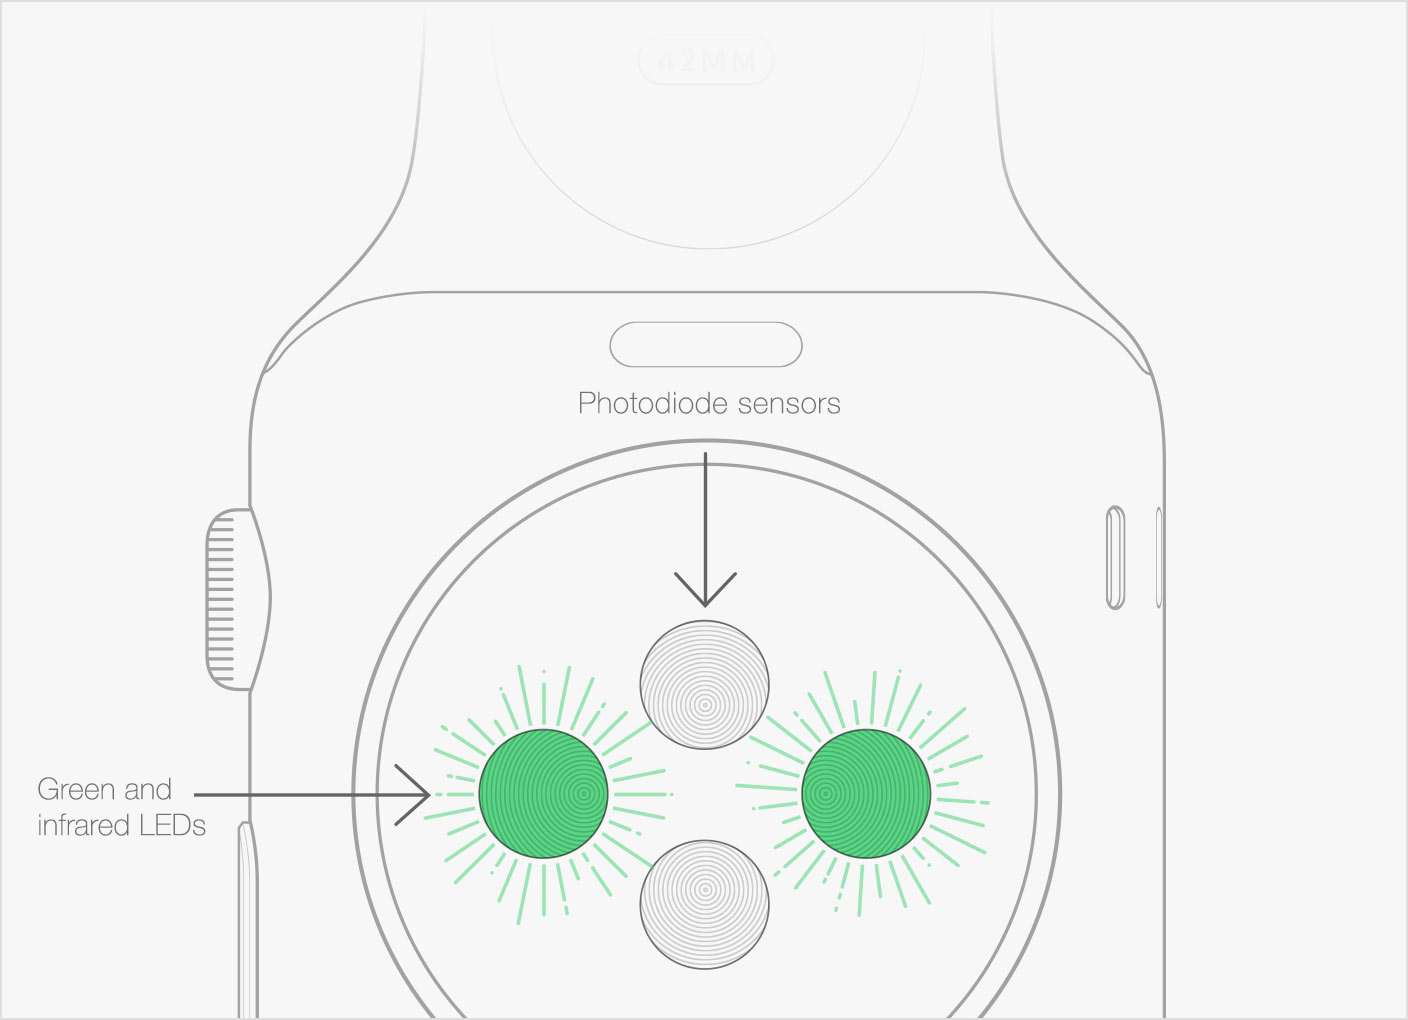
\includegraphics[scale=0.17]{watch-measure-sensors}
	\captionof{figure}{Illustration of the sensor on an Apple Watch}
	\source{\url{https://support.apple.com/en-us/HT204666}}
\end{figure}
%
Fitbit's PurePulse technology is making use of the PPG technique, and so are the Basis Peak HR and the Microsoft Band II.

Many factors effect the performance of the heart rate sensor. 
If the amount of blood flowing through your skin is too low, the heart rate sensor will not get an accurate reading. 
Motion also plays a role: irregular movements decrease the accuracy of the sensor. 
Tattoos can also block the light emitted by the sensor.


\subsection{Heart Rate Variability} \label{section:HRV}
Heart rate variability (HRV) is the variation in the time interval between heartbeats.
It can be measured by measuring the time interval between consecutive heartbeats.
To get a better understanding of this, we take a look at the ECG of a normal sinus rhythm which can be seen in \Cref{fig:ECG}. In this figure, we also see the so-called QRS complex.
In an ECG, the electrical activity of the heart is measured.
The QRS complex is related to the depolarization of the left and right ventricles. 
By some complex processes (that are out of the scope of this thesis), this depolarization eventually causes both ventricles to contract, resulting in a heartbeat. 
By measuring the interval between two consecutive QRS complexes in an ECG, one can determine the HRV.
%
\begin{figure}
	\centering
	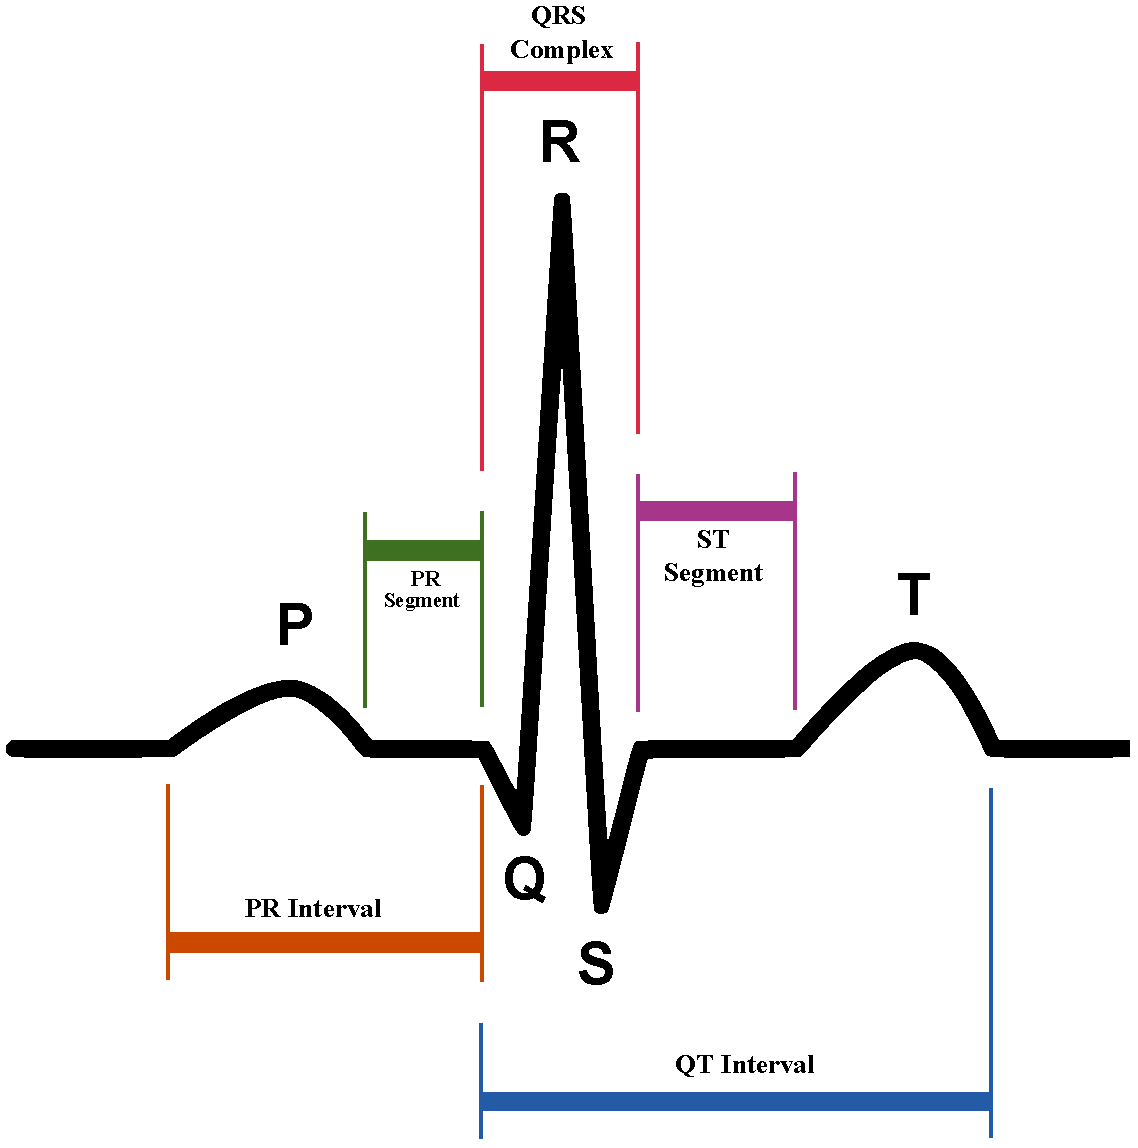
\includegraphics[scale=0.45]{ECG}
	\captionof{figure}{Schematic representation of a normal ECG.}
	\source{Wikipedia}
	\label{fig:ECG}
\end{figure}
%
HRV has proven to be a reliable reflection of the autonomic nervous system, blood pressure and can also be related to gender, sex, age, sleep and diabetes \cite{acharya2006heart}.
The measurements of HRV can generally be grouped under time-domain and frequency domain methods \cite{task1996heart}.
In time domain methods, either the heart rate at any point in time or so called normal-to-normal (NN) intervals between consecutive QRS complexes are determined.
NN is used to make clear that the beats are `normal' beats.
HRV is also referred to as RR variability, where R is the point on the QRS complex.
Some examples of variables that can be calculated when time domain methods are used are the mean heart rate, shortest and longest NN interval and standard deviation.

In frequency domain methods, the heart rate variance is partitioned into underlying rhythms that occur at different frequencies.
Fast Fourier Transform (FFT) is commonly used to find these underlying rhythms.
When this is done, frequencies can be associated with different periodic rhythms.
There are three different rhythms, each with their own frequency range:
%
\begin{itemize}
	\item Very low frequency (VLF) (0.0033 - 0.04 Hz);
	\item Low frequency (LF) (0.04 - 0.15 Hz);
	\item High frequency (HF) (0.15 - 0.4 Hz).
\end{itemize}
%
Afterwards, the NN intervals in each frequency range are counted.

In \cite{thayer2012meta}, HRV as a biomarker for stress was investigated with a meta-analysis of studies.
It was already found that individuals with a greater ability to regulate emotion had greater levels of resting HRV \cite{appelhans2006heart}.

HRV could give more insight in the amount of stress a person is experiencing.
If HRV is a potential biomarker for stress, it must be related to the perception of threat and safety, which are elements of stressors.
That this relation exists was found in \cite{hjortskov2004effect}, where the effect of stress from computer work on HRV and blood pressure was investigated.
Twelve female students participated in the study. They had to perform a computer task where random numbers had to be entered using the keyboard.
The experiment consisted of three stages, in which the participants had to perform the described computer task.
In two of these stages, the experimenter was unfriendly towards his colleagues and unsupportive to the participant. In these stages, the participants also had to perform a memory test.
In the other stage, the experimenter was friendly and supportive, thus eliminating (almost) all stressors.
In this stage no memory test was performed.
Before and after the work, the participants filled in a questionnaire containing a scale to measure the experienced amount of stress.
In stressful situations indicated by the participants, it was found that there was a reduction in the high-frequency component of HRV (calculated from ECG recordings).
An increase in the low- to high-frequency ratio was also found in stressful situations.
The stressors also led to an increase in blood pressure.
This research gives a promising indication for the application of HRV as a biomarker for stress.
In \cite{patel2011applying}, a direct relation was found between the HRV spectrum and fatigue.
In this study, neural network analysis was applied on HRV to assess the fatigue of drivers.
Although the dataset was limited, they managed to get an accuracy of 90\% in predicting whether a given subject was in an alert or in a fatigued state.

\subsection{Two-Minute Walk Test}
During the period of the pilot, MS patients that are participating in our experiment will be asked to do a two-minute walk test (2MWT) every day.
Walking tests are generally used to monitor the effectiveness of a treatment for patients.
The two-minute walk test is a shorter measure of walking performance than the six-minute walk test (6MWT). 
The 2MWT addresses some limitations of the 6MWT.
The latter can be too fatiguing for older people and too time consuming in general.
Especially the limitation of the 6MWT as being too fatiguing, that is addressed in the 2MWT, is relevant for MS patients \cite{gijbels2011comparison}.
Because nerve damage can leave muscles stiff or weak, MS patients can experience a reduced ability to move.
Most of the MS patients also experience fatigue.
Some studies have been done where the measurement properties of the 2MWT were examined \cite{connelly2009clinical} and the reliability and performance was evaluated \cite{bohannon2015two}.
The walking test forces the user to be subjected to physical exertion. 
Therefore, the test can be representative for factors like motivation and fatigue which in turn could be related to day prediction.
In \cite{motl2008worsening}, it was found that a worsening of the symptoms of MS may lead to a reduction of physical activities.
This link could be made visible using the data from the walk test.

As mentioned before, participants will also perform the 2MWT walking test in our experiment.
This will be done using the `Mijn Kwik' app.
This app will record the GPS coordinates as the participants perform the walking test.
The walk test will be initiated as a notification on the phone of the patient.
Only if the GPS accuracy is high enough, the walking test can be started.
This will be explained in more detail in \Cref{section: 2MWT}.

\subsection{Stress} \label{subsection: Stress}
Stress is the response to a stressor. 
A stressor can be an external stimulus or a specific condition in the environment that causes stress.
For humans, stress can be positive or negative. 
Although some forms of stress can have a positive effect on the performance, stress is mostly referred to in a negative way.
Several studies have shown that stress affects MS.
In \cite{buljevac2003self}, researchers investigated the relation of relapsing-remitting MS patients, that experienced attacks, with self-reported stressful events not related to MS.
It was found that the experience of at least one stressful event in a period of four weeks would double the risk of an attack within the next week.
That stress would play an important role in MS has been assumed for a long time.

Some wearables are able to measure the perspiration. 
This is done by measuring  changes in the conductivity of the skin, also called electrodermal activity (EDA), which is related to your sweat production.
The production of sweat is controlled by the sympathetic nervous system.
EDA is related to arousal.
Arousal is the activation state of the autonomic nervous system. 
This is related to the degree of mental awareness or consciousness. 
If the sympathetic nervous system, a branch of the autonomic nervous system, is highly aroused, more sweat will be released resulting in better conductance of the skin.
It will also lead to an increased heart rate and blood pressure.
In addition to motivating certain behaviors like the flight or fight response, arousal also plays an import role in emotion and performance.
Several tasks require different levels of arousals for the best performance.
For example, motivation dependent tasks require higher levels of arousal and concentration dependent tasks require lower levels of arousal for better performance.

In \cite{knufinke2012measurement}, the potential of EDA to measure arousal in a real life setting during exercise was researched. 
This was done using the Affectiva Q\textsuperscript{\texttrademark} sensor that was developed in \cite{poh2010wearable}. This sensor is designed to continuously measure EDA during everyday activities. 
While the measurement of heart rate can also be used to measure levels of arousal, heart rate is influenced by energy demand. Therefore, heart rate is only useful for the measurement of arousal in a resting state, in which energy demand is not influencing the heart rate.
\cite{knufinke2012measurement} illustrated that the measurement of arousal can be done in a high intensive real life setting, which is very promising for daily use of this sensor for MS patients.
%http://www.psychfysio.nl/3_12_2/Arousal is also intertwined with stress.

\subsection{Sitting, Walking and Lying Pattern}
Most of the activity trackers nowadays are able to determine which activity you are doing right now. These activities include walking, running and walking.
We can go into more detail by also keeping track of sitting, walking and lying patterns.

Fatigue is a common symptom for MS patients. 
Researchers have identified the characteristics of so called MS fatigue, that differs from normal fatigue \cite{msfatique}.
These characteristics of fatigue include:
%
\begin{itemize}
	\item Occurring on a daily basis;
	\item Coming easily and suddenly;
	\item Being generally more severe than normal fatigue.
\end{itemize}
%
We could use data from the wearables to get more insight in the pattern of sitting, walking and lying. 
This gives insight in the degree of functional ability and the level of activity during the day.
This could be related to the feeling of a person.
Several studies have researched the classification of activities. 
In \cite{sharma2008frequency}, data from a triaxial accelerometer sensor was used for activity classification.  
The algorithm used for classification was able to classify running, walking and resting activities. 
According to the authors, the algorithm could be extended to also classify activities like standing and sitting.
That this is possible was shown in \cite{karantonis2006implementation}, where a real-time movement classifier was created that could classify activities including falling, sitting, lying (including positions) and standing.
The data being used was collected using a waist-mounted triaxial accelerometer. 
Because the classification was done in real time, the following constraints had to be satisfied:
%
\begin{itemize}
	\item No knowledge of future events;
	\item Amount of buffered data is limited;
	\item Limited processing time: the device must be able to handle the continuous flow of incoming data.
\end{itemize}
% 
When using this data for assessing the quality of upcoming days, the real-time constraints described before are not compulsory.
Data can be send in batches to the database, from which the data can be fetched and used for data mining.
In the described experiment, these real-time constraints led to some limitations of the developed system.
However the experimental results showed that the system was able to classify most activities with a high accuracy.

\subsection{Weather} \label{section:Weather}
That weather can influence your mood is something that many people have experienced. 
That this is no coincidence is confirmed by several studies.
\cite{howarth1984multidimensional} related multiple mood and weather variables.
In this study, it was found that weather was a major predictor for changes in mood. 
For example, a high humidity had a dominant influence on multiple mood variables: 
%
\begin{itemize}
	\item Decrease of concentration and potency;
	\item Increase of sleepiness and fatigue.
\end{itemize}
%
Because some weather data is freely available on the internet, it can be used easily for assessing day quality.
During a meeting with MS patients organized by Orikami, it was found that some patients were more at ease during the summer, while others experienced the same during cold periods.
Heat sensitivity of MS patients is something that has been subjected to extensive research.
In \cite{krupp1988fatigue}, fatigue in MS was investigated. 
This was done by conducting structured interviews with 32 people having MS and 33 healthy adults. 
There were several questions about the characteristics of their fatigue, one of which was ``Heat worsens it". 92\% of the MS patients answered this question with `yes'.
Increased body temperature also seems to influences MS patients. 
In \cite{avis1995sudden}, two cases were described in which heat exposure resulted in death for two patients having MS.
In these cases, exposure to sun (and therefore heat) led to incapacitation of the patients, resulting in death.
Although heat can enlighten the symptoms of MS, it can thus be very dangerous by causing sudden collapses of the thermoregulatory system.

\subsection{Biorhythm}
The theory of biorhythm claims that our life is influenced by rhythmic cycles.
The theory is an example of pseudoscience, which means that it is presented as scientific but does not adhere to the scientific method.
According to the biorhythm theory, three different cycles oscillating in a sine wave (\Cref{fig:biocycles}) influence three different aspects of our life \cite{hines1998comprehensive}. 
The three cycles are:
%
\begin{itemize}
	\item A 23 day cycle that influences \textbf{physical} aspects of behavior. 
	The equation for this cycle is $\sin(2\pi t/23)$.
	
	\item A 28 cycle that influences \textbf{emotions}.
	The equation for this cycle is $\sin(2\pi t/28)$.
	
	\item A 33 day cycle that influences \textbf{intellectual} functions. 
	The equation for this cycle is $\sin(2\pi t/33)$.
\end{itemize}
%
\begin{figure}
	\centering
	\begin{tikzpicture}
		\begin{axis}[domain=0:21*pi, samples=100,grid=major,
			restrict y to domain=-3:3,xlabel=$t$,ylabel=$y(x)$, legend pos=outer north east]
			\addplot [color=green]    	{sin(deg(x)*2*pi/23};
			\addplot [color=red]  		{sin(deg(x)*2*pi/28};
			\addplot [color=blue] 		{sin(deg(x)*2*pi/33}; 
			\legend{Physical, Emotional, Intellectual}
		\end{axis}
	\end{tikzpicture}
		\captionof{figure}{Biorhythm of the first 66 days after birth.}
		\label{fig:biocycles}
\end{figure}
%
In each of the equations, $t$ indicates the number of days since birth.
According to modern biorhythm theory, these cycles start at the moment of birth and proceed to exist during the rest our lives. 
The durations of these periods do not change.
The required knowledge to apply this theory gives us a great advantage.
By only having knowledge of an individual's date of birth, one is able to calculate the position on each cycle of a particular person, giving insight in the current state for each of the cycles. However, the theory of biorhythm remains controversial.
No scientific evidence has been found that supports the theory.
Some researchers even claim that it has no more predictive power than chance.
It might be worth using biorhythm as a biomarker for day quality, despite its restricted expressive power.

\subsection{Fatigue}
Questionnaires in general can help to retrieve useful information from the user.
The `Mijn Kwik' app, which is also used for the 2MWT experiment, contains questionnaires as well.
The corresponding questions can be seen in \Cref{fig:app} in \Cref{section: Data storage}.
An example of such a question is the slider that can be used by a patient to indicate how energetic he is feeling right now.
Such a question is just one indicator.
There is no simple measure to determine if someone is fatigued, there are just different ways of estimating the level of fatigue.
Below we will discuss several scales that could be used in questionnaires.

\paragraph{Visual Analogue Scales}
Visual Analogue Scales (VAS) can be used as a psychometric response scale in questionnaires. 
It consists of a straight line, where each end of the line contains an extreme statement.
These statements are two opposite claims, for example the statements `no pain' and `the greatest pain I can imagine'. 
In the case where the patient must indicate how he is feeling today (\Cref{fig:app:mood} in \Cref{section: Data storage}), this scale is also used.
A problem with this method is that it is hard to make a distinction between all the possibilities.
The choice made can only be partly explained by the underling property, making it hard to spot measurement errors.
Due to its simplicity, VAS can easily be used.
However, attention must be paid to its role.
It should never be used alone, due to its biases \cite{torrance2001visual}:
%
\begin{itemize}
	\item Context Bias: a VAS score for a state depends on the number of better and worse states that are present at the same time.
	If a state is included with more states that are better, its value is depressed.
	This is in contrast with the effect that occurs when a state is included with more states being worse: its value is enhanced.
	
	\item End-aversion Bias: this bias refers to the reluctance of some respondents to use the extreme values of the scale, or to use the ends when using a continuous scale.
	
\end{itemize}
%

\paragraph{Samn-Perelli Seven Point Fatigue Scale}
The Samn-Perelli Seven Point Fatigue Scale (SPS) is a 7-point scale with scores ranging from 1 (``fully alert, wide awake'') to 7 (``completely exhausted, unable to function effectively'') \cite{samn1982estimating}, which has been validated and is being used widely.

\paragraph{Karolinska Sleepiness Scale}
The Karolinska Sleepiness Scale (KSS) can be used to evaluate sleepiness. 
It has been validated against EEG activity and is also widely used.
KSS is a one-dimensional scale with scores ranging from 1 (``very alert'') to 9 (``very sleepy, great effort to keep awake'').\\

As we can see, there are a lot of verified techniques to get a measurement of fatigue.
Which technique is the best in this setting could be determined by using these scales throughout the pilot and asking feedback from the participants.  


\subsection{Sleep} \label{section:Sleep}
Sleep is a very important stage of the day in our lives. 
While sleeping, our body comes to rest.
For humans (generally for mammals), sleep can be divided in two types: rapid eye movement (REM) and non-rapid eye movement (NREM).
Each of these types have characteristic features.

\paragraph{REM}
During the REM phase in sleep, there is an increased brain activity compared to when being awake.
The muscles in the body are completely relaxed and the eyes make horizontal and vertical movements. Only during this phase of sleep, people are able to dream.
While sleeping, an adult remains on average 15\% of his sleep in REM phase.
Although it is not completely clear what the function of REM sleep is, there are several hypotheses about the functions of REM sleep.
In general, sleep helps to save memories.
Thus, REM might play a role in the processes that make sure that our memories are stored in our memory (memory consolidation), however REM is not a necessary condition for this process.

In \cite{tsoukalas2012origin}, a totally different theory is proposed, which states that REM sleep evolved out of a defensive reflex called toxic immobility. 
This reflex results in total immobilization of an animal, which creates the suggestion that the animal is dead.
This reflex is useful as a last line of defense when the animal is attacked by a predator.
According to this theory, this reflex has similarities with REM sleep.

\paragraph{NREM}
In this stage of sleeping, there is hardly any eye movement.
In contrary to REM, dreaming is rare in this stage of sleeping and there is no relaxation of the muscles. NREM can be divided in three stages \cite{schulz2008rethinking}. While transitioning from the first to the second stage, the movement of the eyes is reduced. In the last stage, it is more common to fall asleep than in the other stages.

As with the theories for REM, there also exist a lot of theories about the function of sleep:
%
\begin{itemize}
	\item Increases the restoration of the body;
	\item Contributes to the processing of memories;
	\item Dreaming, that can occur during some sleep stages, can help processing experiences.
\end{itemize}
%
When researchers want to get insight in the sleep of one or several persons, sleep studies are conducted. 
A common sleep study is polysomnography (PSG), which is also the gold standard for evaluating a person's sleep.
During this sleep study, the following will be measured \cite{polysomnography}:
%
\begin{itemize}
	\item Oxygen in blood;
	\item Eye movement;
	\item Heart rate;
	\item Brain waves;
	\item Activity of muscles;
	\item Lying position;
	\item Amount of air you breathe in and out.
\end{itemize}
%
Most of these measurements cannot be done with simple activity trackers, but they do provide detailed information about a night of sleep.
This information is based on the movements in your sleep.
At the end of the night, these movements are fed into algorithms that calculate sleep scores based on your relative amount of movement during the night. 
Although they can be a good indicator for your amount of sleep during the day, the quality for some other related measurements are not verified.
This is especially the case for complex information like the time you spend in (N)REM during the night, for which it is unknown how these sleeping states are determined.
Often a sleep score is assigned to a night of sleep.
Some activity trackers show how this score is calculated, but it is hard to say how representative this score is. 
Sleep duration however is something that could be useful when looking at good or bad days.

\subsection{Vitamin D}
Vitamin D plays a very interesting role in the risks of relapses for MS patients. 
It is already known that vitamin D is an environmental factor that plays a role in the development of MS.
In \cite{runia2015multiple}, the relation between vitamin D levels and the risk in relapsing-remitting MS of an exacerbation (a synonym for a relapse) was investigated in a longitudinal study with 73 patients having RRMS. 
It was found that higher levels of vitamin D were associated with a decrease in the risk of exacerbations. 
Vitamin D appears to suppress the autoimmune response of T cells attacking the myelin sheaths of the nerve cells and axons.
When vitamin D was given in a high dose to MS patients, the activity of the T cells dropped significantly.
However, some studies suggest that there is an opposite relation between vitamin D and a decreased risk of exacerbation in MS patients: low vitamin D levels are caused by less time spend outside due to increased disabilities for MS patients \cite{van2007vitamin}.
Vitamin D levels can be influenced by sunlight.
The effectiveness of exposing the skin to sunlight, and thereby `getting' vitamin D, depends on several factors:
%
\begin{itemize}
	\item \textbf{Color of the skin}. People with a darker skin tone tend to produce less vitamin D when being exposed to sunlight.
	\item \textbf{Time of the day}. Ultraviolet B rays (UVB) play a role in the natural way of getting vitamin D. 
	When the sun is shining on the earth at a large angle, these UVB rays are blocked. 
	Thus during early and late parts of the day, exposing your skin to the sun will not help in the synthesis of vitamin D.
	\item \textbf{Where you live}. The closer you live to the equator, the easier it will be for your body to synthesize vitamin D from UVB rays. 
\end{itemize}
%
It was already known that vitamin D had a protective effect at the start of MS, but new research shows that it can also effect the course of the disease. 
With the data from wearables, it might be possible to get an approximation of the time spent outdoors.
Because time spent outdoors can influence vitamin D levels, the chance or increased risk of an exacerbation could be determined.

\subsection{Neurogenesis} \label{subsection: Neurogenesis}
Neurogenesis is the name of the process responsible for growing new neurons.
The hippocampus is a place in the brain of the human body where new neurons can be created.
Neurogenesis plays an important role in learning, memory, mood and emotion \cite{smithimpact}.
What is also mentioned in this research, is that there is a clear relation between neurogenesis and depression.
A reduced adult hippocampal neurogenesis (AHN) in different animal models, where antidepressants were able to restore this, is supporting this relation \cite{malberg2003cell, dranovsky2006hippocampal}.
It is also possible to influence the process of neurogenesis. 
In \cite{stangl2009impact}, an overview of different diets, and their influence on AHN for rats and mice was given.
Diets consisting of high saturated fat, were found to reduce the production of new neurons. The same effect was found for the intake of ethanol, that is present in alcohol.
Intermittent fasting and reducing your calorie intake were found to increase neurogenesis.
This effect was also found for foods with a soft texture.

Despite the fact that a lot more factors influence depression and mood, in theory it would be possible to predict levels of depression based on someones diet.
This would make it possible to prevent the effect of stress and even prevent depression.
Because the evidence for the mediation of AHN on the effect of diets on mental health is limited, more studies are needed to confirm this relation. 
In \Cref{table:effectsneurogenesis}, the effect on neurogenesis for some activities or events is given.
%
\begin{table}
	\centering
	\begin{tabular}{@{}ll@{}}
		\toprule
		\multicolumn{2}{l}{\textbf{Effect on neurogenesis}} \\
		\cline{0-1}
		\textbf{Increases} & \textbf{Decrease}  \\ \midrule
		Running & Aging\\
		Sex & Sleep deprivation\\
		Learning & Stress \\ \bottomrule
	\end{tabular}
	\captionof{table}{Events that increase or decrease neurogenesis \cite{thuret2015grow}.}
	\label{table:effectsneurogenesis}
\end{table}
%
% !TeX spellcheck = en_US
% !TeX root = ../MS_analysis_thesis.tex

\section{Selecting Relevant Biomarkers} \label{section:Selecting Relevant Biomarkers}
As we have seen in \Cref{section:relevant biomarkers}, there is a large collection of biomarkers that could be related to good and bad days. In this section, we will identify which biomarkers could be useful. 
This will be done by looking at the use of biomarkers in other diseases for longer periods of time. 
We must also look at current technology being able to measure the biomarker.

\subsection{Limiting the Set of Relevant Biomarkers}
There are couple of biomarkers for which we decided they could not be used in our research.
This applies to the following biomarkers: vitamin D, weather, neurogenesis, stress, `sitting, walking and lying pattern' and HRV.
We do actually see potential for each individual biomarker in future research.
However, currently those biomarkers are not easy to measure, have not been investigated thoroughly, have not been used in practice or cannot be measured by consumer-available devices.
All of these reasons made us choose a specific selection of biomarkers.
Before looking into this selection, we will describe for each of these biomarkers listed above why we decided not use them in our research.
%
\begin{itemize}
	\item For measuring vitamin D, we would need some sort of advanced sensor that could determine the amount of vitamin D in the blood. 
	Although such devices exist, this would force our participants to manage multiple devices simultaneously. 
	This would add unnecessary complexity.
	While writing this thesis, there did not actually exist any consumer-available device that could measure vitamin D (as far as we know).
	All these reasons made us not to choose this biomarker.
	
	\item Neurogenesis is a new research topic that is currently being explored.
	As we have seen in \Cref{subsection: Neurogenesis}, certain kind of activities and foods are influencing this process.
	Because the topic is relatively new, there is no data from which we can see how a certain type of food or activity influences neurogenesis. 
	If this data was present however, this would require more user intervention: users would need to input their meals into the application.
	This seems undesirable.
	This observation of unwanted complexity ruled out neurogenesis as a biomarker.
	
	\item As seen in \Cref{subsection: Stress}, stress and arousal are partly intertwined. 
	We have seen that the measurement of sweat on the skin using a dedicated sensor can be used to measure levels of arousal. 
	Some activity trackers are able to measure this sweat production on the skin, but not all of them. 
	Because the functionality was not present on all the activity trackers we had available for our experiment, we chose not to include this biomarker.
	
	\item Activity classification is something that most activity trackers can do.
	However, the classification of positions (sitting / walking / lying pattern) is not a basic functionality for currently available activity trackers.
	Due to this currently lacking feature of activity trackers, we decided not to include this biomarker as well.
	
	\item Weather data is freely available, and given that most patients prefer certain temperatures this is a promising biomarker. Due to time restrictions, we decided not to include this biomarker in our research.
	
	\item Despite the restricted knowledge on HRV, it appears to be a reliable biomarker for responses to stress. 
	While acute stress only influences HRV for a short term, chronic stress can even affect HRV during sleep. 
	This was found in \cite{hall2004acute}. 
	These stress related changes in HRV caused significant decreases in sleep maintenance, which is the ability to remain at sleep during night.
	Thus, the effects of some forms of stress on HRV can be seen for an extended period of time. 
	Despite being a very useful biomarker, HRV cannot be measured using current available smartwatches.
	It requires advanced technology like ECG to get an accurate approximation of HRV.
	It is very likely that smartwatches in the future will have the ability to measure this indicator accurately.
	However, due to the current restriction of technology available for consumers, we will not select this biomarker.
\end{itemize}
%

\subsection{Selected Biomarkers}
Fatigue seems to be one of the most common symptom of MS.
The results from the \textbf{2MWT} can be used as a reliable and valid measure of the physical function of patients. 
This is only possible when the test is standardized.
A problem with the 2MWT is that there is a lack of reference values.
This limits the interpretation of the results.
In \cite{selman2014reference}, this limitation was addressed by establishing a reference equation to predict the distance walked in the 2MWT.
This was done for healthy participants.
The equation was as follows:
%
\begin{align*}
\text{2MWT}_{\text{predicted}} &= 252.583 - (1.165 \times \text{age}) + (19.987 \times \text{gender}^*) \\
& \text{gender}^* = 
\begin{cases*}
1 & \text{if } \text{male}\\
0 & \text{if } \text{female}
\end{cases*}
\end{align*}
%
The equation was found to be highly reproducible in healthy subjects.
It might be possible to come up with an equation for MS patients that is capable of giving an estimation of the distance walked. 
This equation could have additional parameters, like the type of MS the patient has and the current severity of the disease.

Standardization of the 2MWT in the pilot is something that requires some more attention.
Because the lack of a supervisor during this test, people might have different expectations on how to perform the walking test.
There is documentation available in the `Mijn Kwik' app about the test, but if people put this text in the same perspective as terms of use, it is not likely that this documentation is read thoroughly.
Despite these uncertainties, the results of these tests seem promising as a potential biomarker.
For MS, both the 6MWT and the 2MWT \cite{gijbels2010predicting} were tested on relevance of habitual walking performance (HBW).
Both the 2MWT and 6MWT were the best predictors among all the other tests for habitual walking performance, confirming its high potential.

Your \textbf{resting heart rate} (RHR) (\Cref{section:Resting Heart Rate}) can be influenced by a lot of factors, including stress.
When being exposed to stress for a long period, your body is constantly functioning in a high gear and therefore affecting your heart rate.
Stress can also reduce your energy, sleep and make you feel cranky.
Stress is also playing a big role in MS (\Cref{subsection: Stress}).
Although the use of resting heart rate from heart rate data from wearables in research is a new concept, it can prove useful.
Combined with data from the questionnaire app, we can take a closer look at the relation between heart rate and the indicated quality of the next day.

There have been some follow up studies on the effect of elevated resting heart rate on the risk of all-cause mortality.
In \cite{jensen2013elevated}, this effect was researched on 2798 healthy middle-aged men in a 16-year follow up study.
An inverse relation was found between resting heart rate (RHR) and physical fitness.
An increased RHR was also related to mortality, independent of the physical fitness of a person

During \textbf{sleep} (\Cref{section:Sleep}), you lay the foundation for your next day.
You will immediately notice the impact of lack of sleep from the previous night.
Sleep also plays an important role in your mood.
In \cite{totterdell1994associations}, the relations between sleep and mood were investigated.
It was found that sleep was more related to subsequent well-being than prior well-being.
Also an earlier onset of sleep was related to a better mood the next day. 
Earlier onset of sleep was also a better predictor of mood than sleep duration.
This seems to be in conflict with the general opinion that duration of sleep has the most impact on your mood.

However, in \cite{rehagen2015short} the effect of a short sleep duration on the intake of nutrients and mood was investigated.
Undergraduate college students were used in this experiment.
It was found that the total mood disturbance (TMD) score was linked to sleep duration and sleep quality. 
The Pittsburgh Sleep Quality Index (PSQI) was used to measure the quality and pattern of sleep. 
It also includes questions to estimate the sleep duration.
Participants that had a sleep duration of at least 6 hours during the night had lower TDM scores $(p = 0.0091)$ and therefore experienced a more positive mood state the next day.
This suggests that a short sleep duration and a lower sleep quality have a negative impact on the mood state.

In \cite{wichniak2013sleep}, sleep as a biomarker for depression was investigated.
Changes in a person's sleep pattern also seem to be important for diagnosing a subtype of depression, regardless of being positive (more sleep or an improvement of sleep quality) or negative (decrease in sleep or worsening of sleep quality).
Sleep (and specifically sleep duration) can therefore be used as a biomarker to determine the increased risk for depression, which influences the quality of upcoming days.
\input{chapters/experiment}
\input{chapters/research}
% !TeX spellcheck = en_US
% !TeX root = ../MS_analysis_thesis.tex

\chapter{Conclusion and Discussion}\label{chapter: Conclusion and Discussion}
\lettrine[lhang = 0.4, findent=-60pt, lines=7]{\textbf{
		\initfamily \fontsize{40mm}{40mm} \selectfont I
		\normalfont}}{n}
this thesis, we have looked at relevant biomarkers in the prediction of good and bad days for multiple sclerosis (MS) patients. 
Because activity trackers were used, the validity and reliability was reviewed in \Cref{section: Reliable Data Collection}.
In this section it was found that activity trackers are widely used in the research field and that the measurement of most of the health related variables are an accurate representation of the true values.
In \Cref{section:relevant biomarkers}, we have conducted a literature review for relevant biomarkers. 
This was done by looking at how biomarkers can be measured and how they are currently being used or could be used to get more insight in the health state of (MS) patients.
In \Cref{section: 2MWT}, two experiments were designed and conducted to test the reliability of GPS coordinates that were used to calculate the distance walked in the 2MWT.
In both experiments it was found that the quality of the GPS tracks would differ a lot.
There were tracks that would give a good approximation of the total distance walked but other tracks were of insufficient quality to get a good estimation.
From the result of the final experiment, it was decided that applying clustering on the GPS points belonging to a GPS track would detect the outliers.
These outliers are excluded in the algorithm for calculating the total distance walked.
After reviewing existing usage of biomarkers in \Cref{section:Selecting Relevant Biomarkers}, we chose the following biomarkers for investigating their relation with good and bad day analysis: 2MWT, resting heart rate (RHR) and sleep duration.
For the results of the 2MWT, the final algorithm which makes use of clustering was used to calculate the distance walked in the analysis of the data from the participants.
For each individual biomarker, we investigated its relation with the day rating of the next day by using statistical analysis.
Although we found some relations that confirmed or refuted some of our hypotheses, their was too much diversity to conclude anything.
The restricted dataset and number of participants contributed to this. 
We also found that some data seemed to be missing and that participants were forgetting to rate days using the `Mijn Kwik' app.
Especially data, that required the participant to perform specific tasks in order to become available, was missing.
To minimize the risk of missing data due to participant in future research, most of the measurement should be done automatically if possible.

Although we focused on a small selection of biomarkers to investigate their potential as a biomarker in the prediction of good and bad days for MS patients, we do not exclude the use of others.
As an example, another biomarker was `found' during a hackathon.
In the weekend of 21-22 May 2016, this MS hackathon was organized in Amsterdam, the Netherlands%
\footnote{\url{http://www.mshackathon.nl}}.
In this hackathon, a variety of people worked together to gain new insights into MS for researchers, doctors and patients themselves.
A team from Orikami also participated in this hackathon.
Currently there is not an objective scale to measure fatigue.
People that have to indicate themselves how fatigued they are, seem to have problems with this: they are not able to correctly make an estimation of their current fatigue.
Relatives however are often able to see when people are fatigued, although these people cannot see this by themselves.
In current literature, the relation between eye movement and fatigue has already been investigated \cite{Arief_2009}.
Based on these findings, we came up with the idea to measure fatigue based on recordings from the eye.
By letting the user focus on a screen on which circles appear randomly, we can determine how fast the eye responds on these events.
Using these measurement, we would like to get an objective measurement of the fatigue level from MS patients.
The idea was also appreciated by specialists and MS patients and we even managed to win the 2nd place.
In the future, this new technique should be investigated even more to get a more accurate measurement on fatigue for MS patients.

Because this thesis can be seen as an exploratory study, the lack of any relation between the investigated biomarkers and the day ratings was in line with our expectations.
In upcoming research, investigating the relation between biomarkers and the quality of upcoming days could be done using more sophisticated methods.
This should also include analysis in which multiple biomarkers are considered at the same time.

\bibliographystyle{plain}
\bibliography{bib/bibliography}

% !TeX spellcheck = en_US
% !TeX root = ../BachelorThesis.tex
\appendix
\numberwithin{figure}{section}
\chapter{Appendix}

\section{GPS Plots Straight Path}
%
\begin{figure}[H]
	\centering
	\subfloat[]{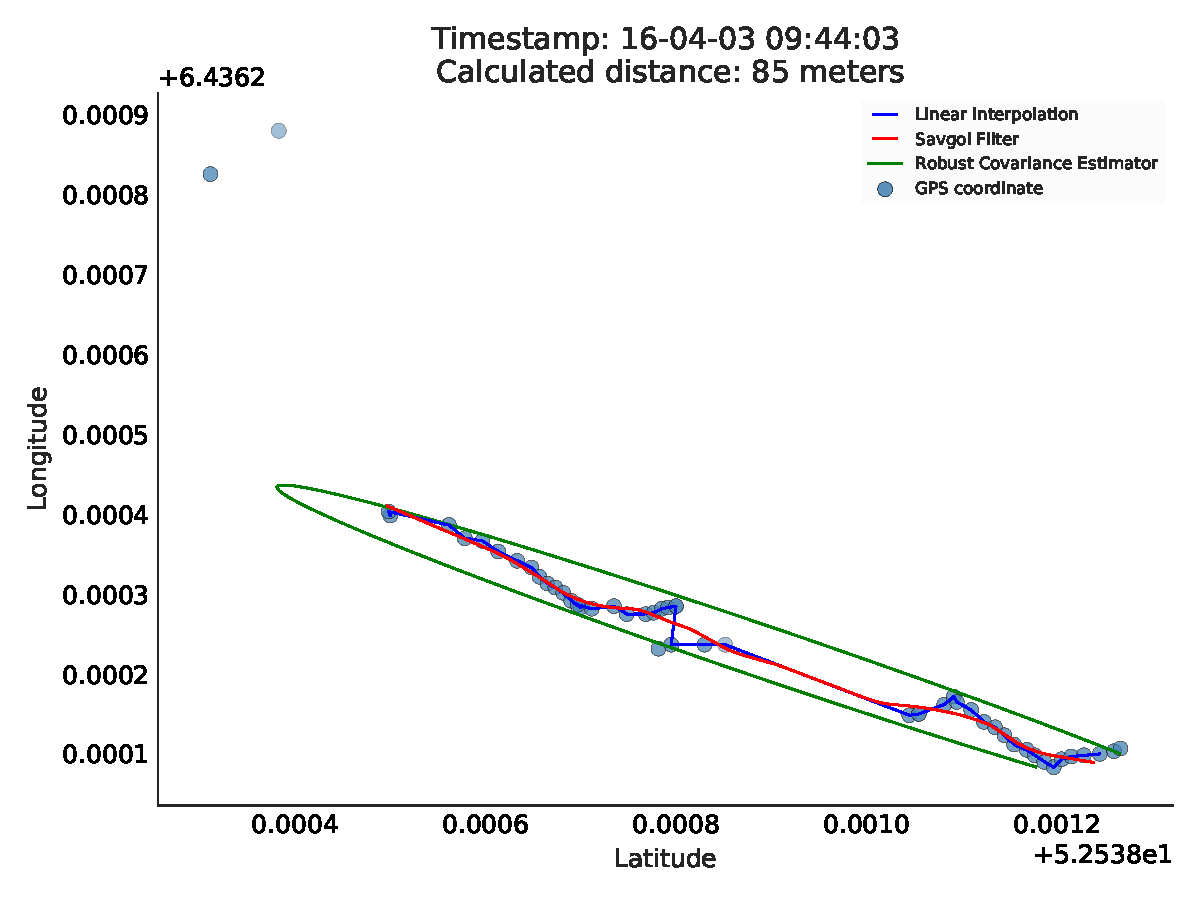
\includegraphics[scale=0.29]{gps/straight/3wAkwQDaLY7gYrhPi}
	}
	\hspace{0.5cm}
	\subfloat[]{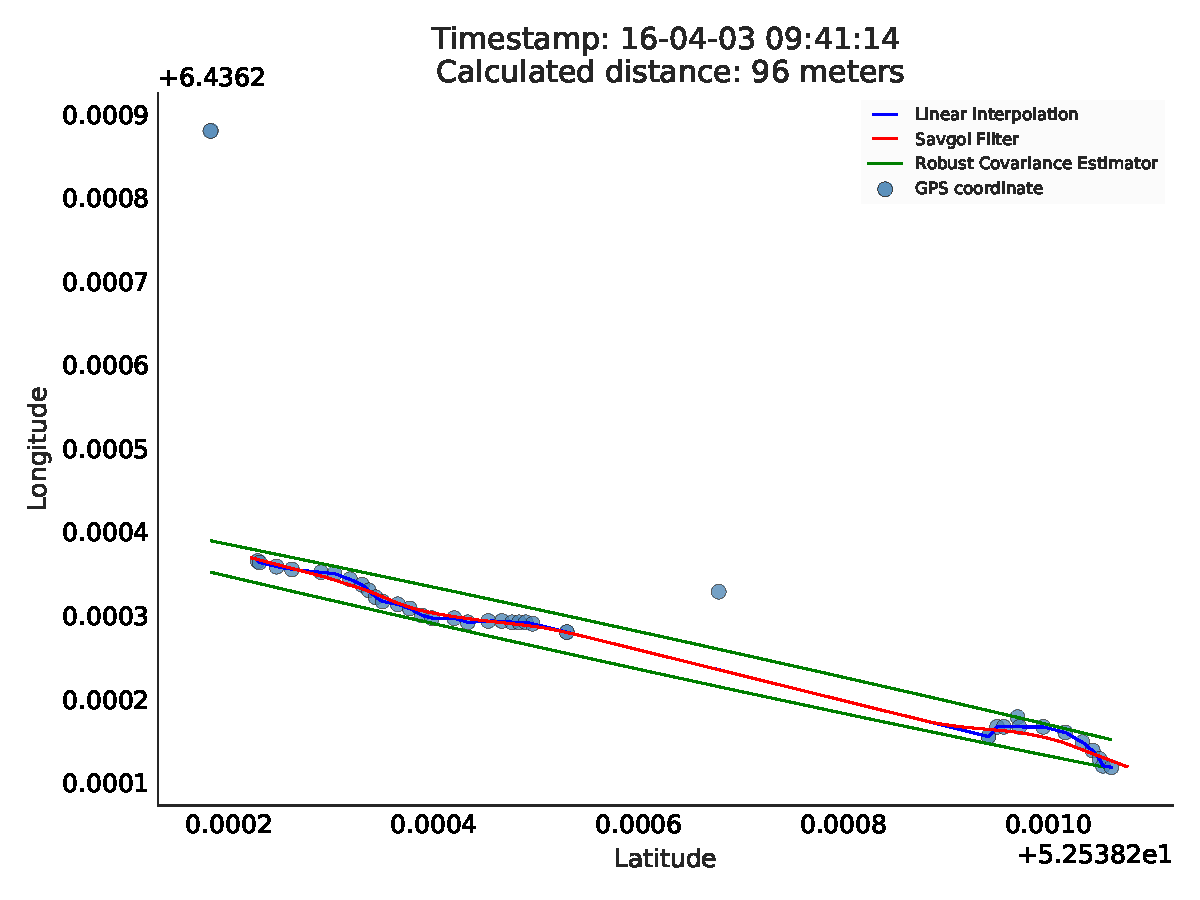
\includegraphics[scale=0.29]{gps/straight/9cuCTXcBBK2J32PoE}
	}
	\vfill
	\subfloat[]{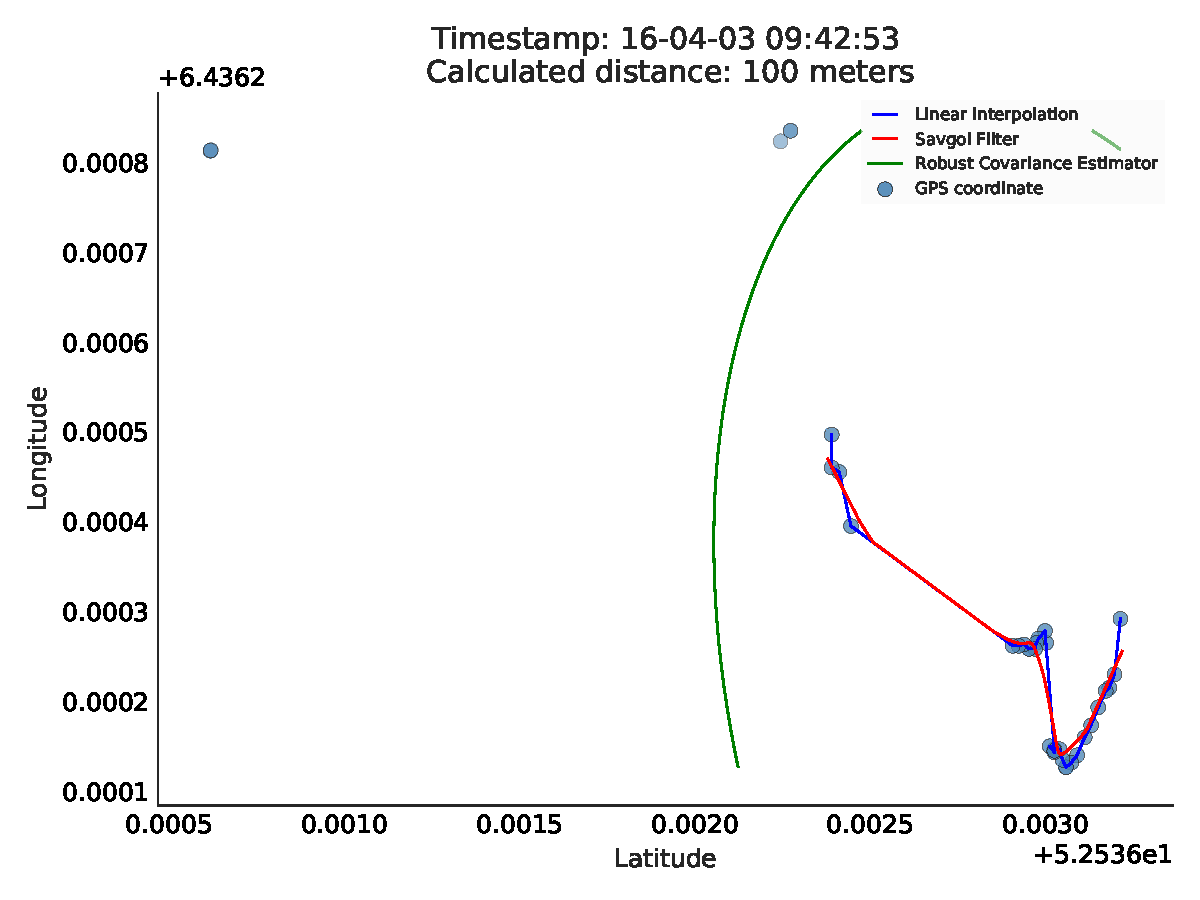
\includegraphics[scale=0.29]{gps/straight/Ba8aoCEfdhz2nxYq9}
	}
	\hspace{0.5cm}
	\subfloat[]{\label{fig:Terrible GPS Coordinates 1}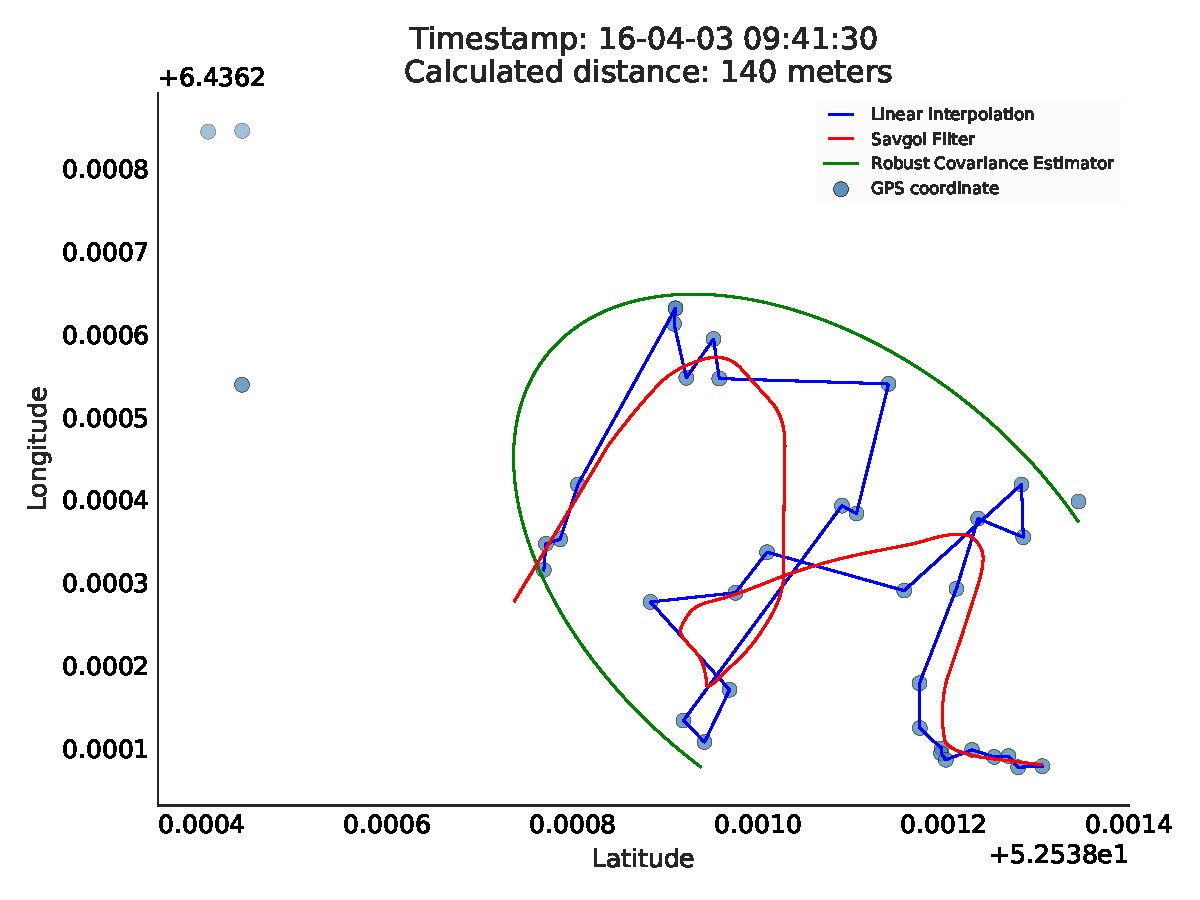
\includegraphics[scale=0.29]{gps/straight/CbpZDcgq8d6BCy5mj}
	}
	\captionof{figure}{Plots of the GPS coordinates of the walking test before and after smoothing. First, outlier detection is done using Elliptic Envelope. Afterwards, inliners are  smoothed in two stages: `Lineair Interpolation' is the first smoothing step and `Savgol Filter' the last.}
	\label{GPS Plots Straight Line}
\end{figure}
%
\begin{figure}[H]
	\ContinuedFloat 
	\centering
	\subfloat[]{\label{fig:Terrible GPS Coordinates 2}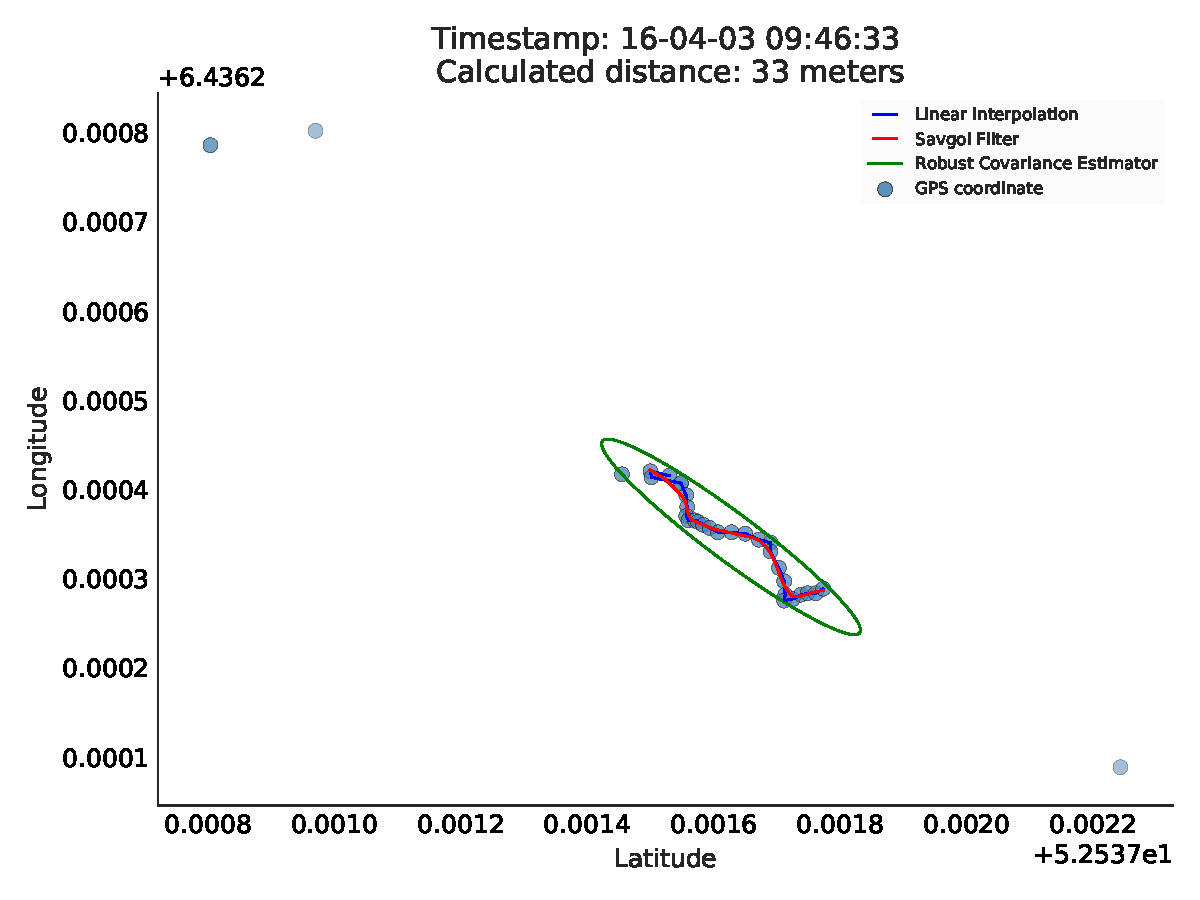
\includegraphics[scale=0.29]{gps/straight/exCkb4K2cCaZHHg4b}
	}
	\hspace{0.5cm}
	\subfloat[]{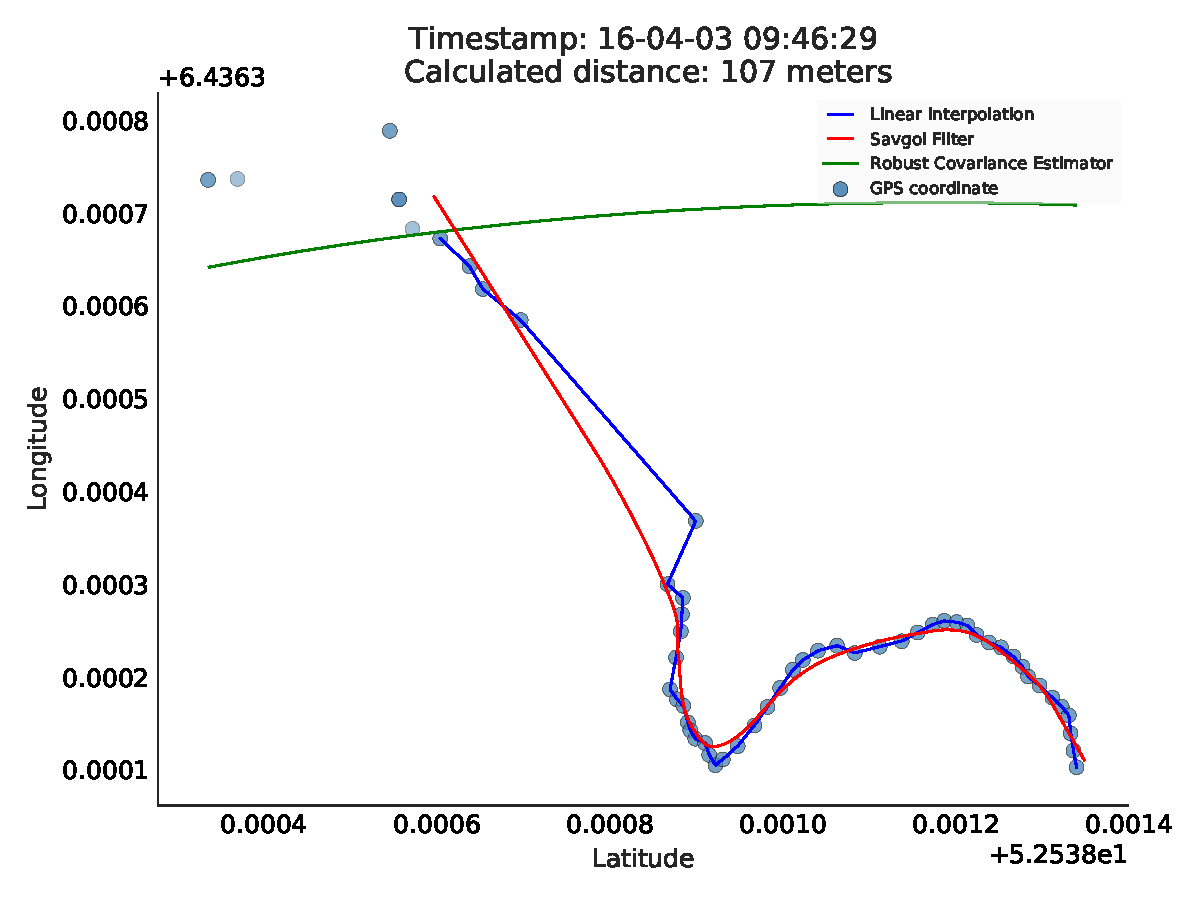
\includegraphics[scale=0.29]{gps/straight/fA2QJHC6iPcAmnu4x}
	}
	\vfill
	\subfloat[]{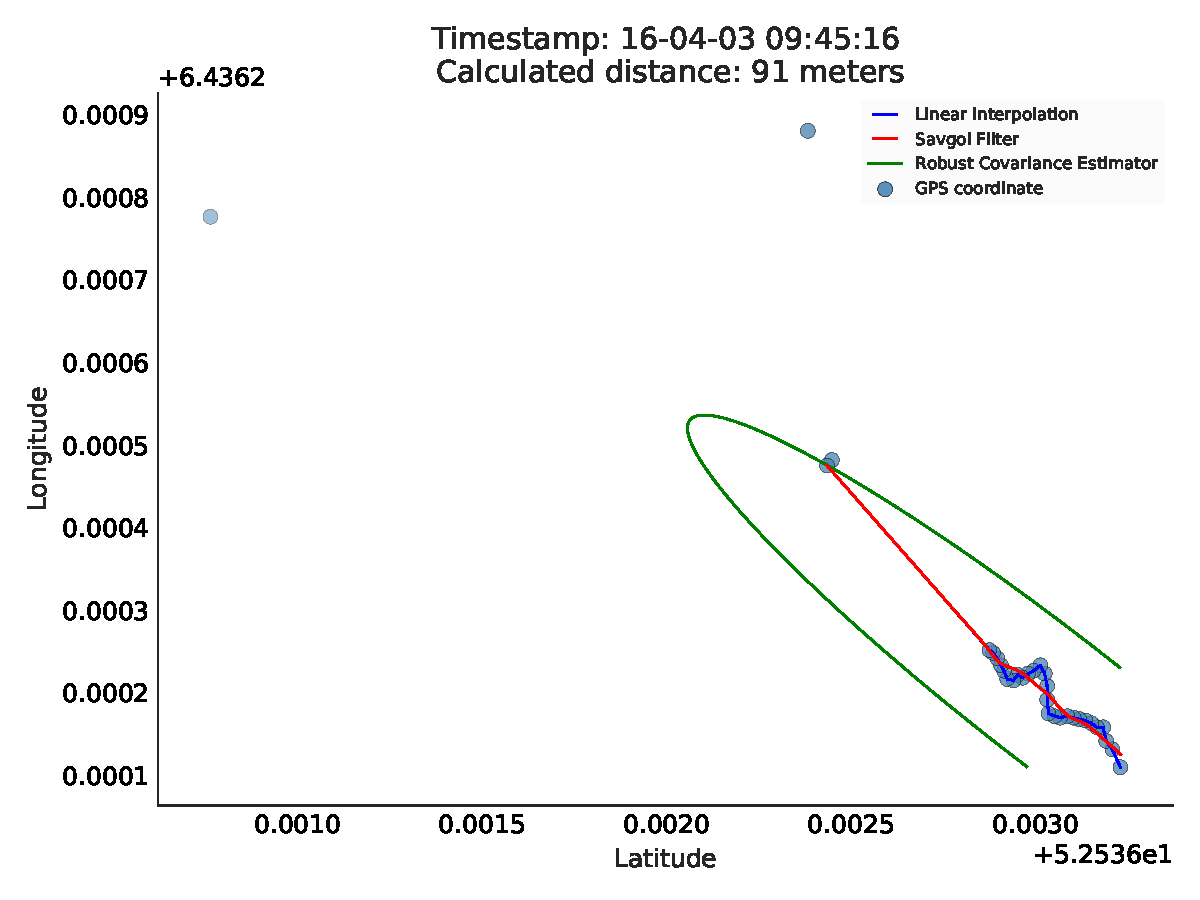
\includegraphics[scale=0.29]{gps/straight/g7zX6A4FnTu4L975N}
	}
	\hspace{0.5cm}
	\subfloat[]{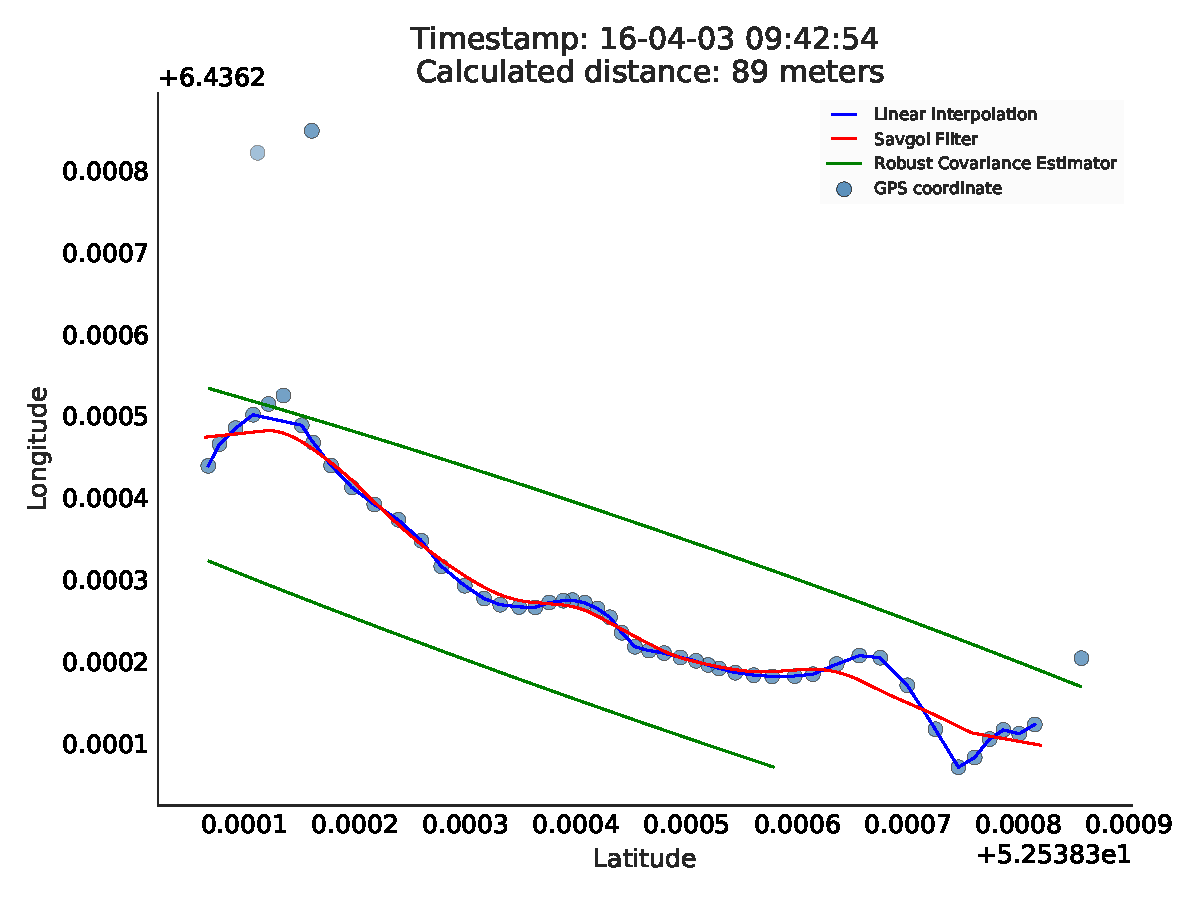
\includegraphics[scale=0.29]{gps/straight/KFb4FtR8Jjb6Ajtdc}
	}
	\vfill
	\subfloat[]{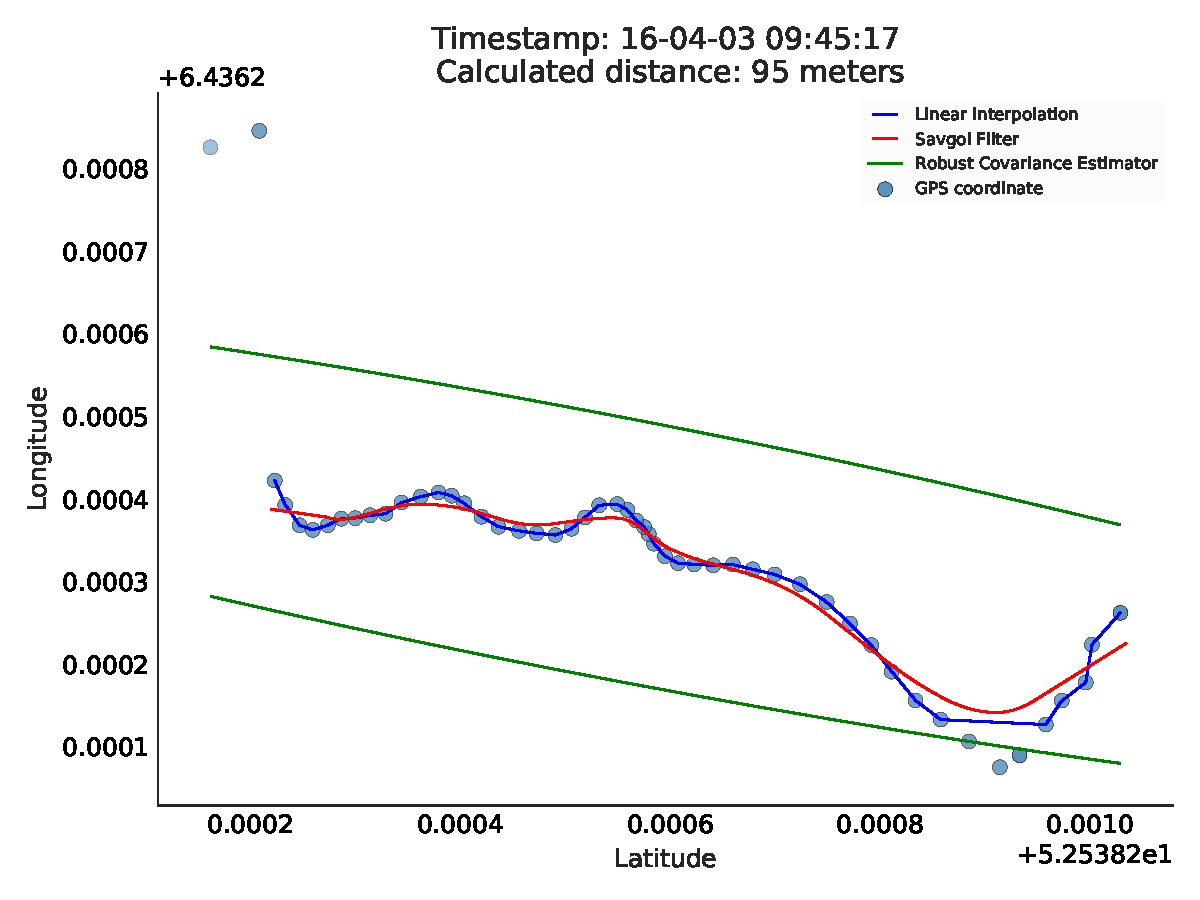
\includegraphics[scale=0.29]{gps/straight/QXtSsihbjmWnG854C}
	}
	\hspace{0.5cm}
	\subfloat[]{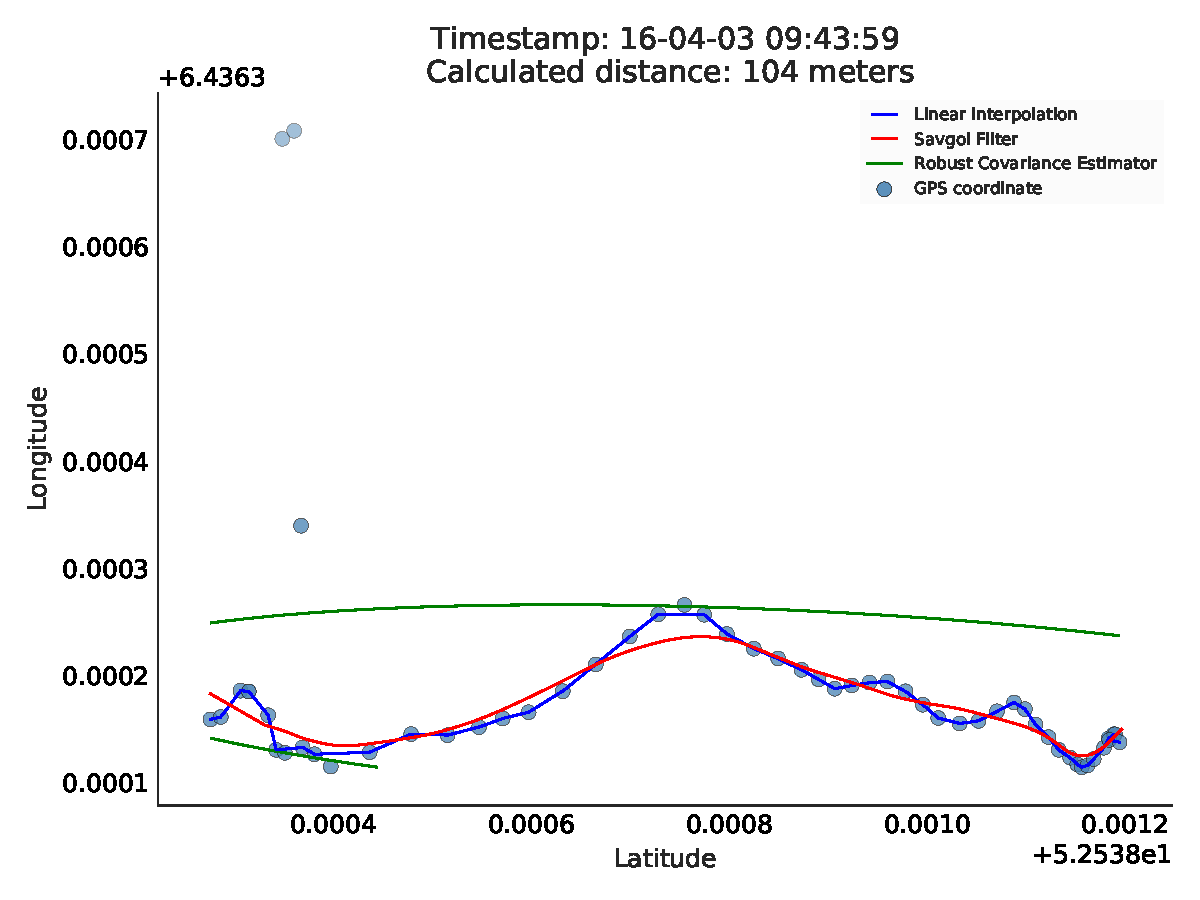
\includegraphics[scale=0.29]{gps/straight/vGn6KLTyNqBEH25YN}
	}
	\captionof{figure}{}
\end{figure}

\newpage

\section{GPS Plots Circular Path}
\begin{figure}[H]
	\centering
	\subfloat[]{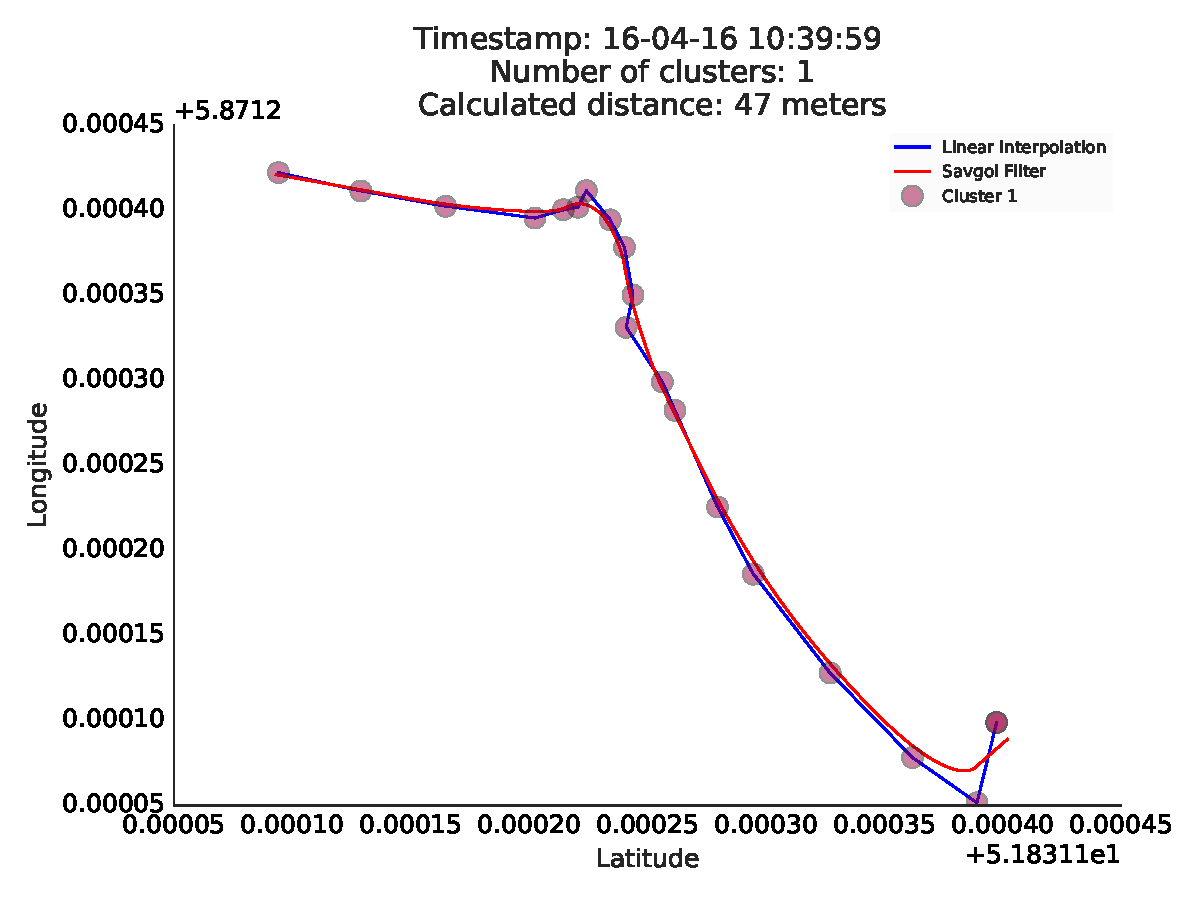
\includegraphics[scale=0.29]{gps/circle/2Zye5dTxYRNq7K7se}
	}
	\hspace{0.5cm}
	\subfloat[]{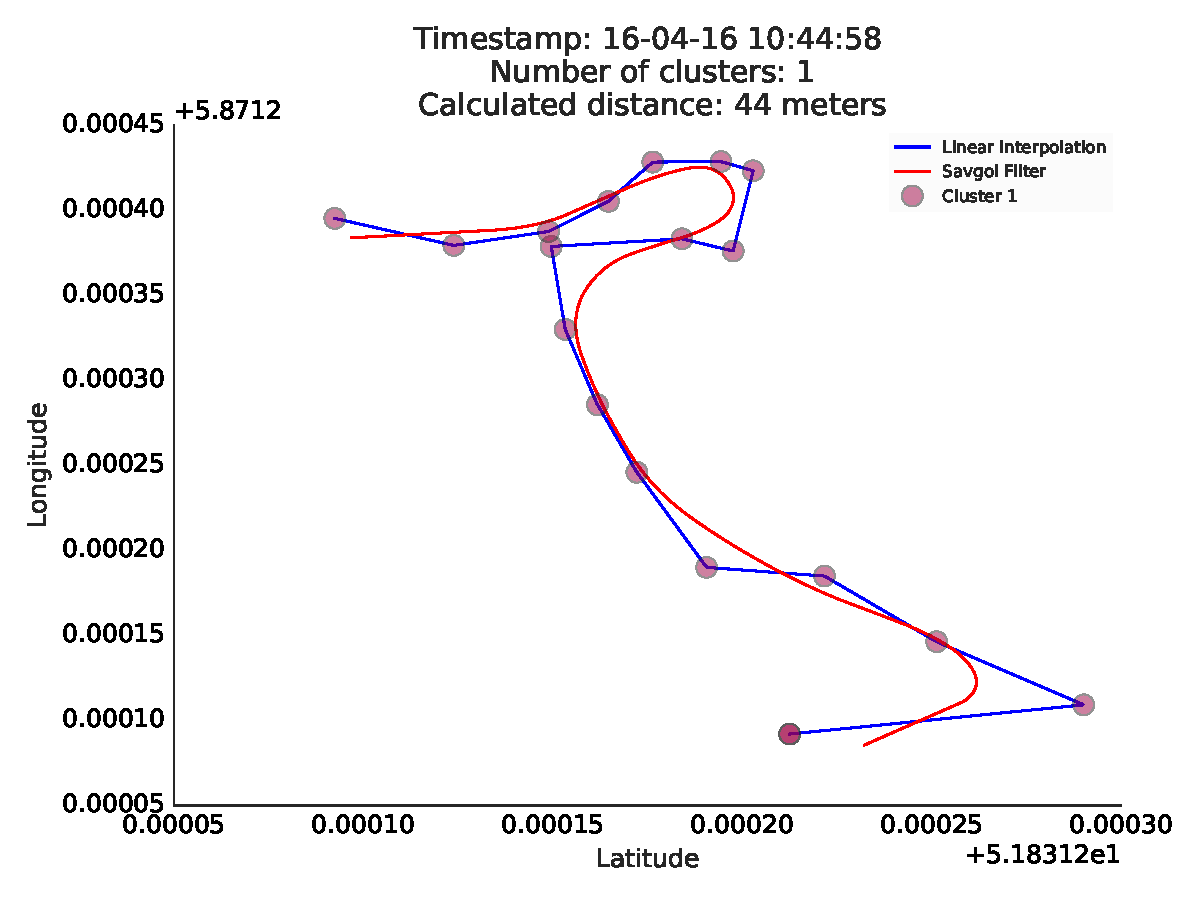
\includegraphics[scale=0.29]{gps/circle/4E2jhxMF392sEjWJF}
	}
	\vfill
	\subfloat[]{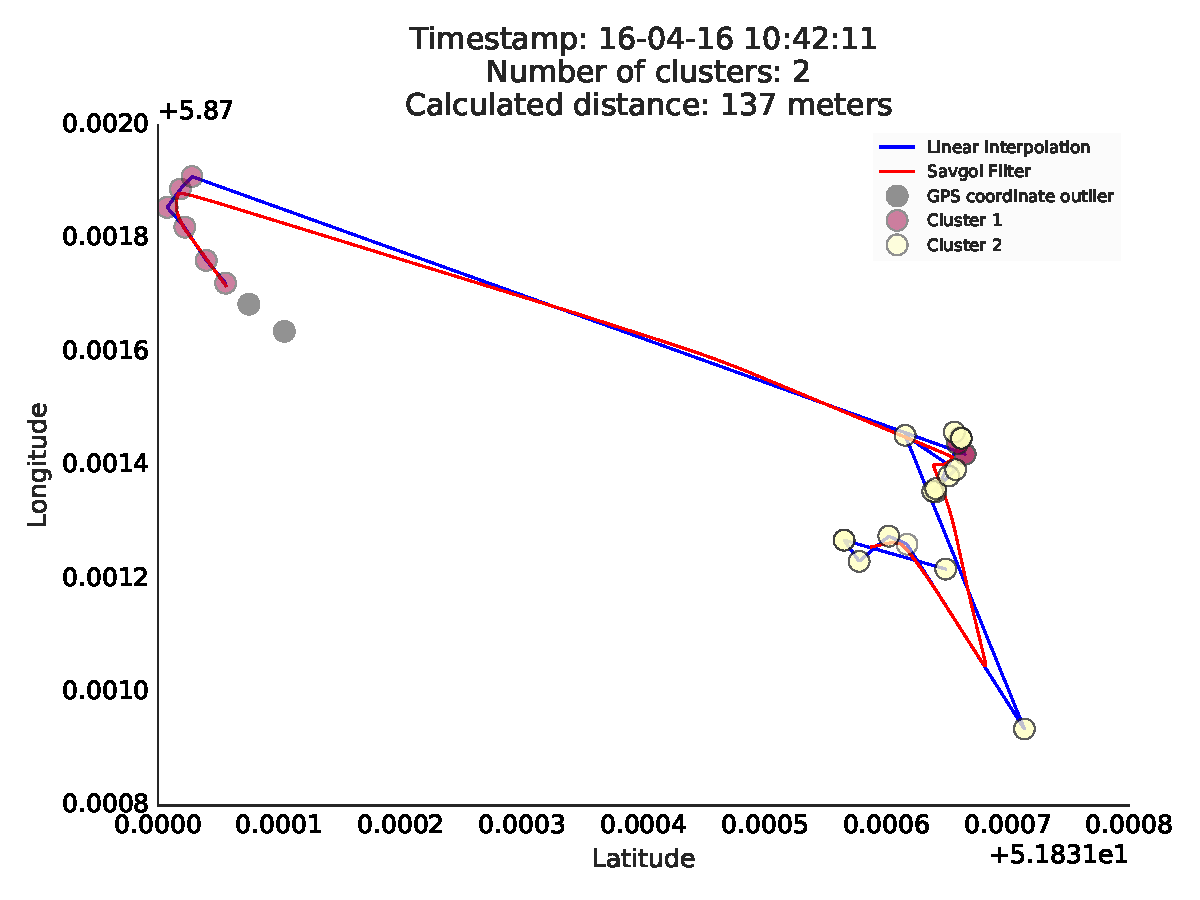
\includegraphics[scale=0.29]{gps/circle/HFgtoEcsXcmiDZHtY}
	}
	% Was eerst 141m door fout, nu 137
	\hspace{0.5cm}
	\subfloat[]{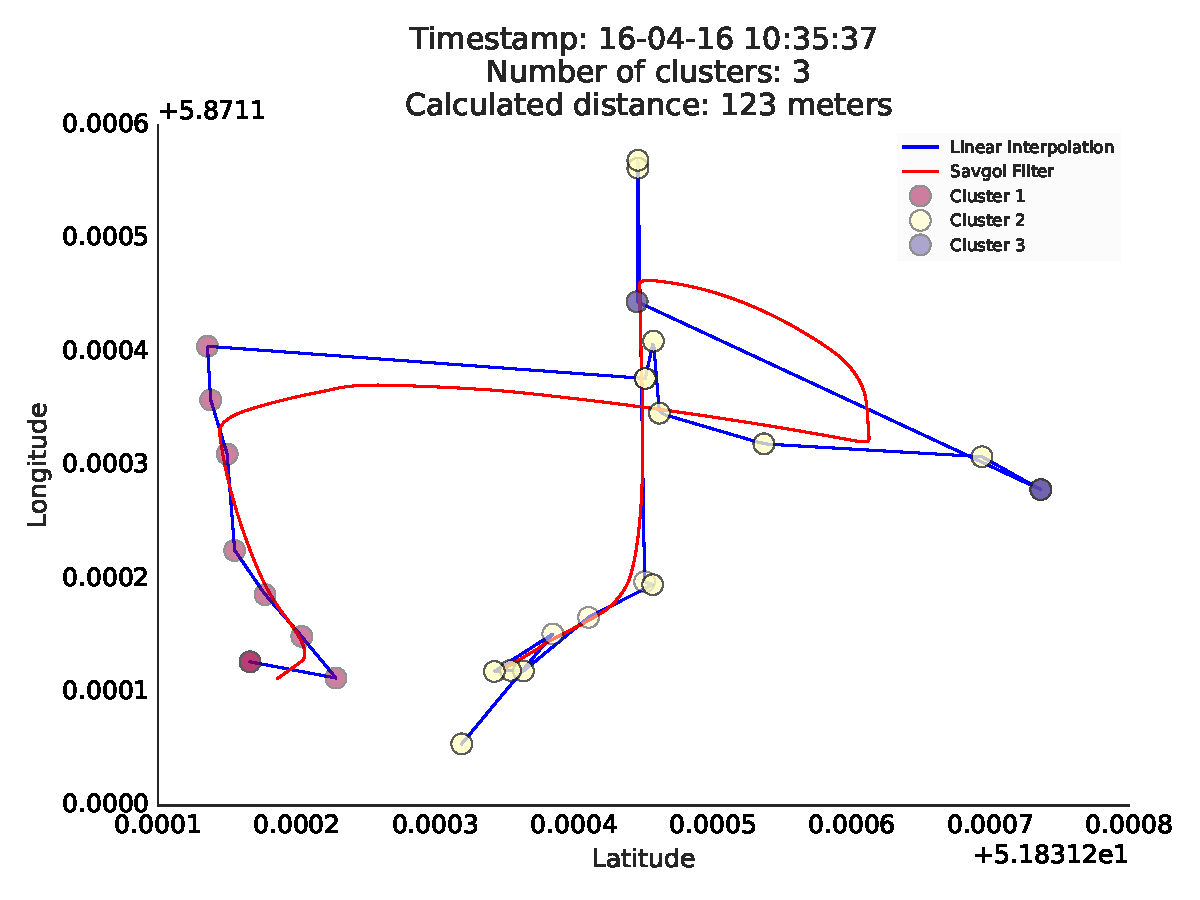
\includegraphics[scale=0.29]{gps/circle/otZE8i4oahYFNdegA}
	}
	\vfill
	\subfloat[]{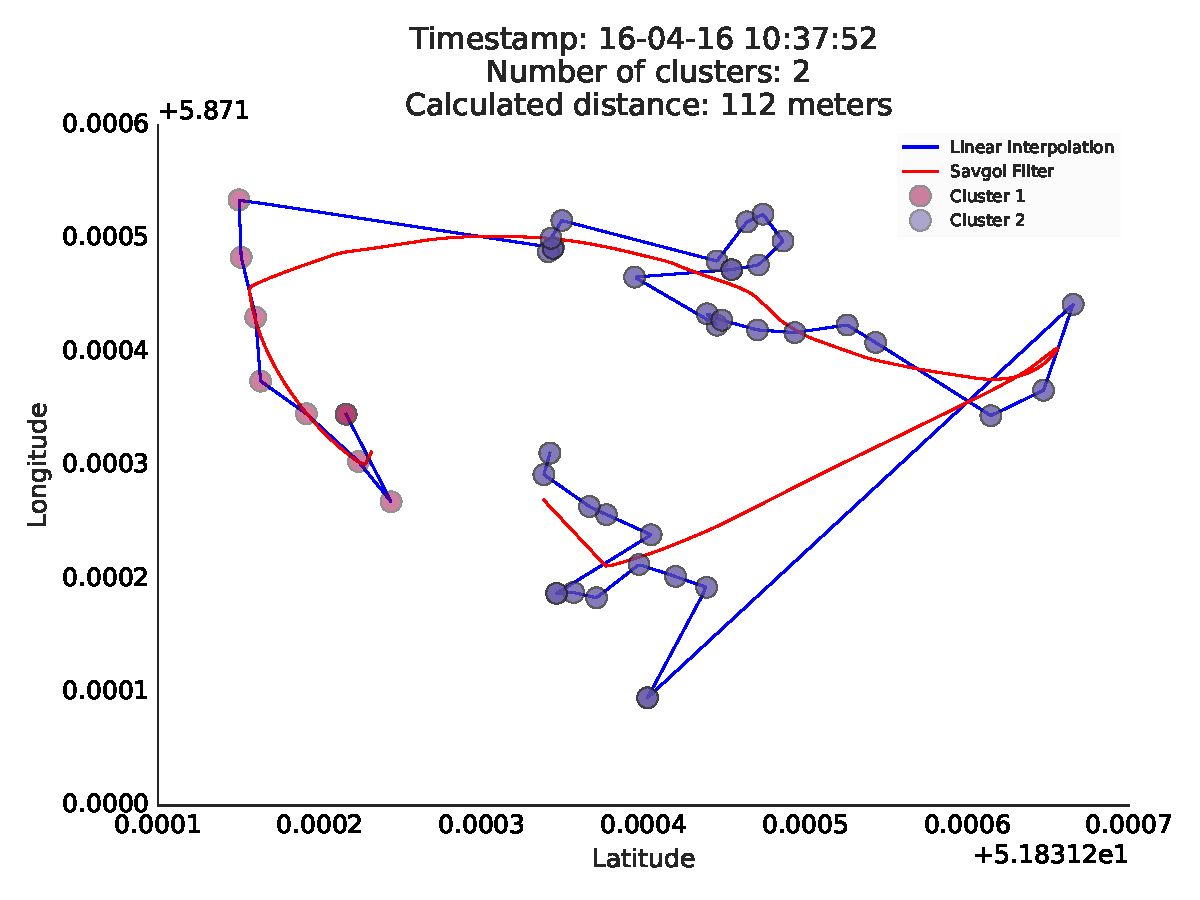
\includegraphics[scale=0.29]{gps/circle/Px5F2nQ9iaYACpJXG}
	}
	\captionof{figure}{Plots of the GPS coordinates of the walking test using a circular track. First, clustering is used to filter out the outliers. Afterwards, inliners are  smoothed in two stages: `Lineair Interpolation' is the first smoothing step and `Savgol Filter' the last. Black points are points classified as noise.}
\end{figure}

\newpage

\section{Heart Rate Boxplots}
\begin{figure}[H]
	\centering
	\subfloat[]{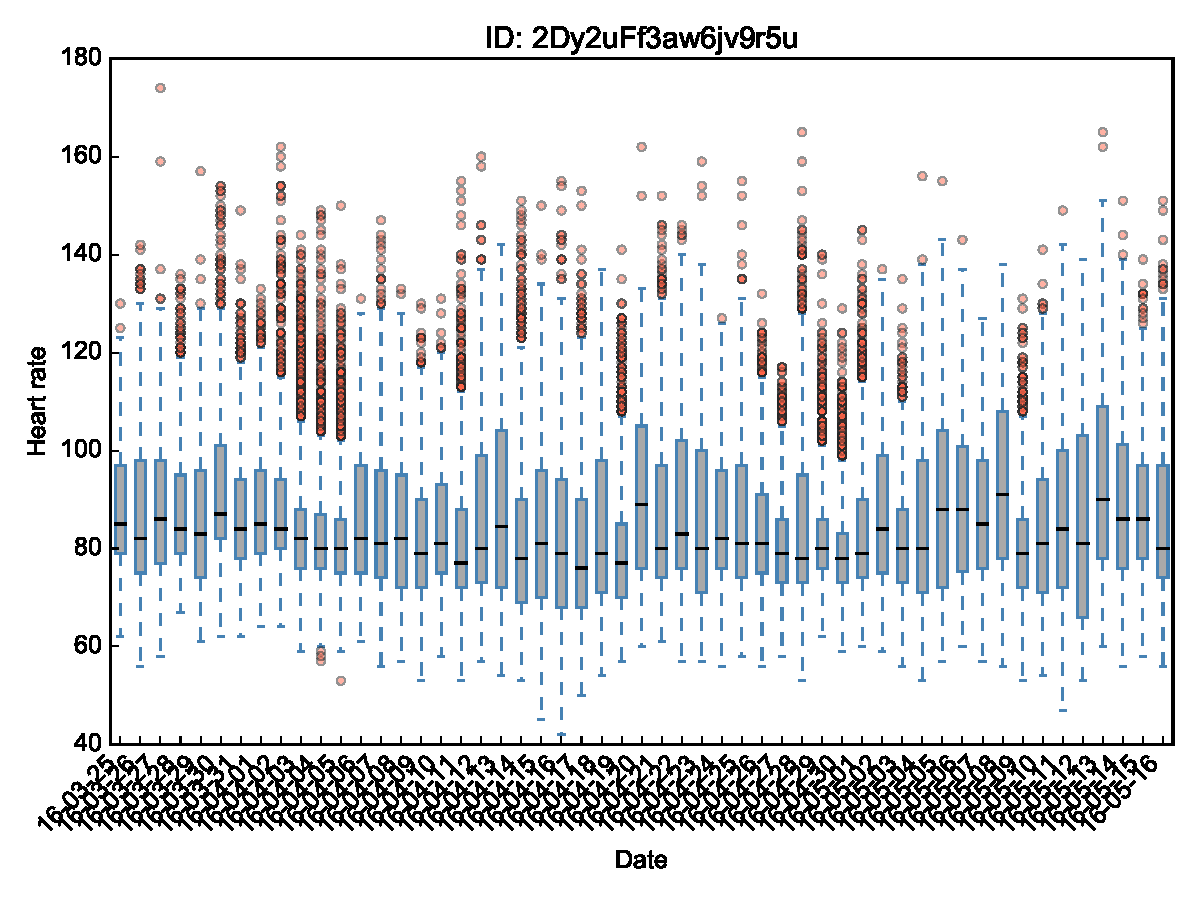
\includegraphics[scale=0.5]{boxplots/2Dy2uFf3aw6jv9r5u}
	}
	\vfill
	\subfloat[]{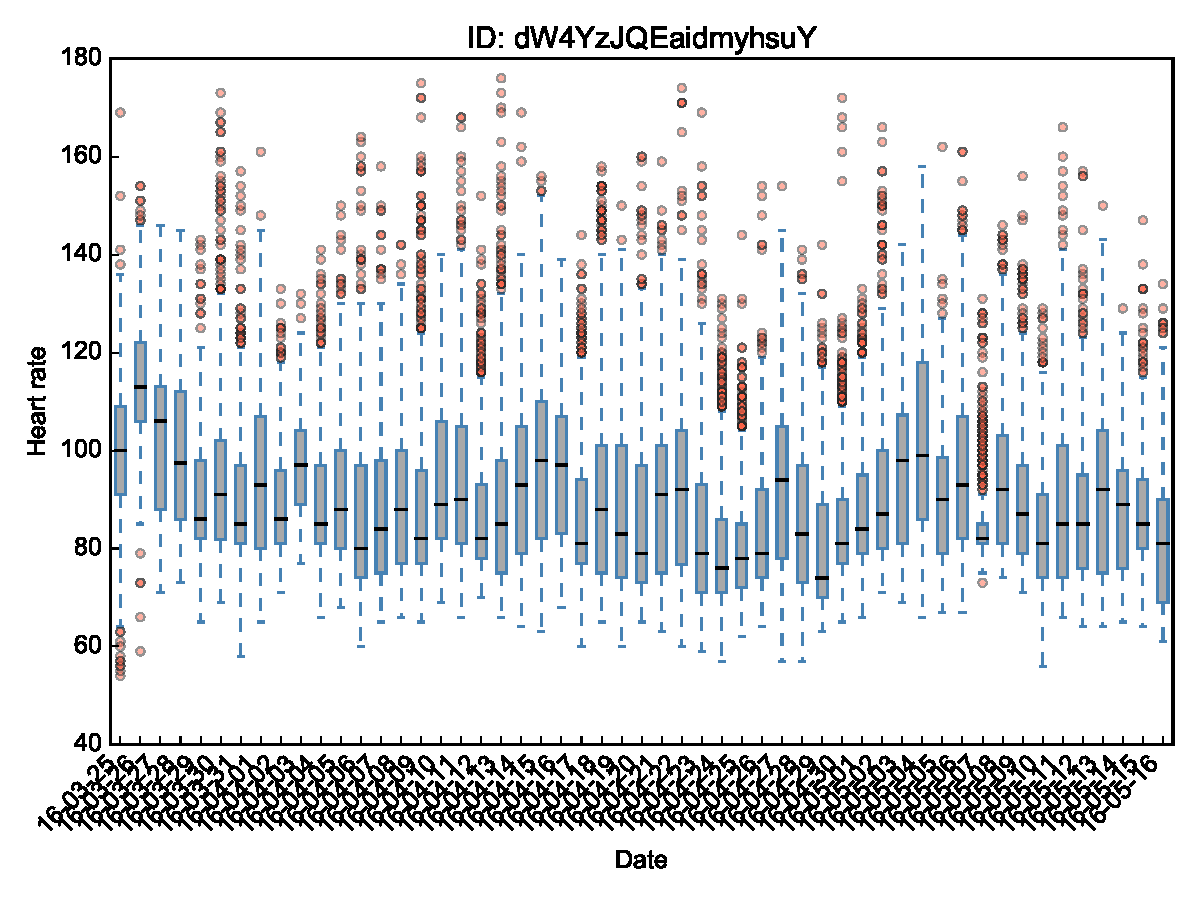
\includegraphics[scale=0.5]{boxplots/dW4YzJQEaidmyhsuY}
	}
	\captionof{figure}{Boxplots of the heart rates for each day.}
	\label{fig: heart rates boxplots}
\end{figure}

\begin{figure}
	\ContinuedFloat
	\centering
	\subfloat[]{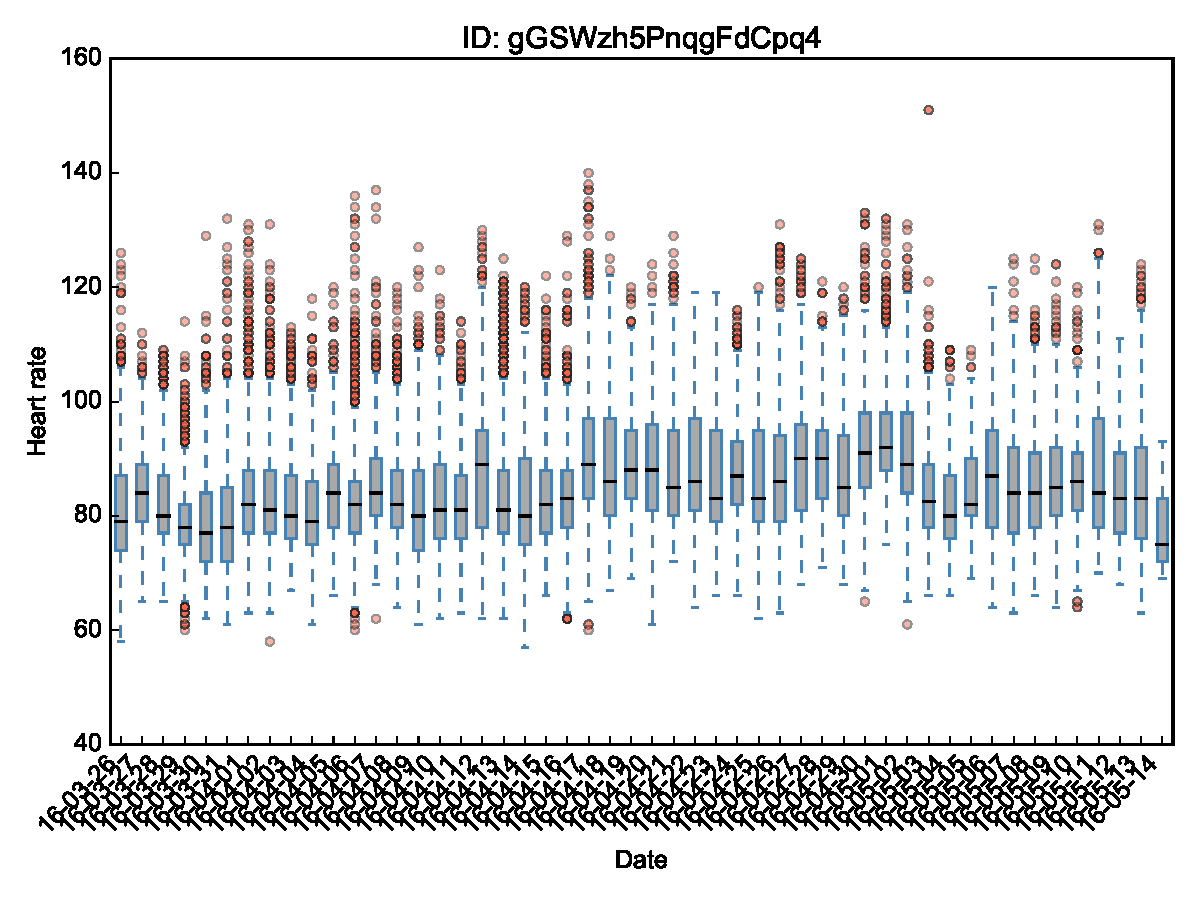
\includegraphics[scale=0.5]{boxplots/gGSWzh5PnqgFdCpq4}
	}
	\vfill
	\subfloat[]{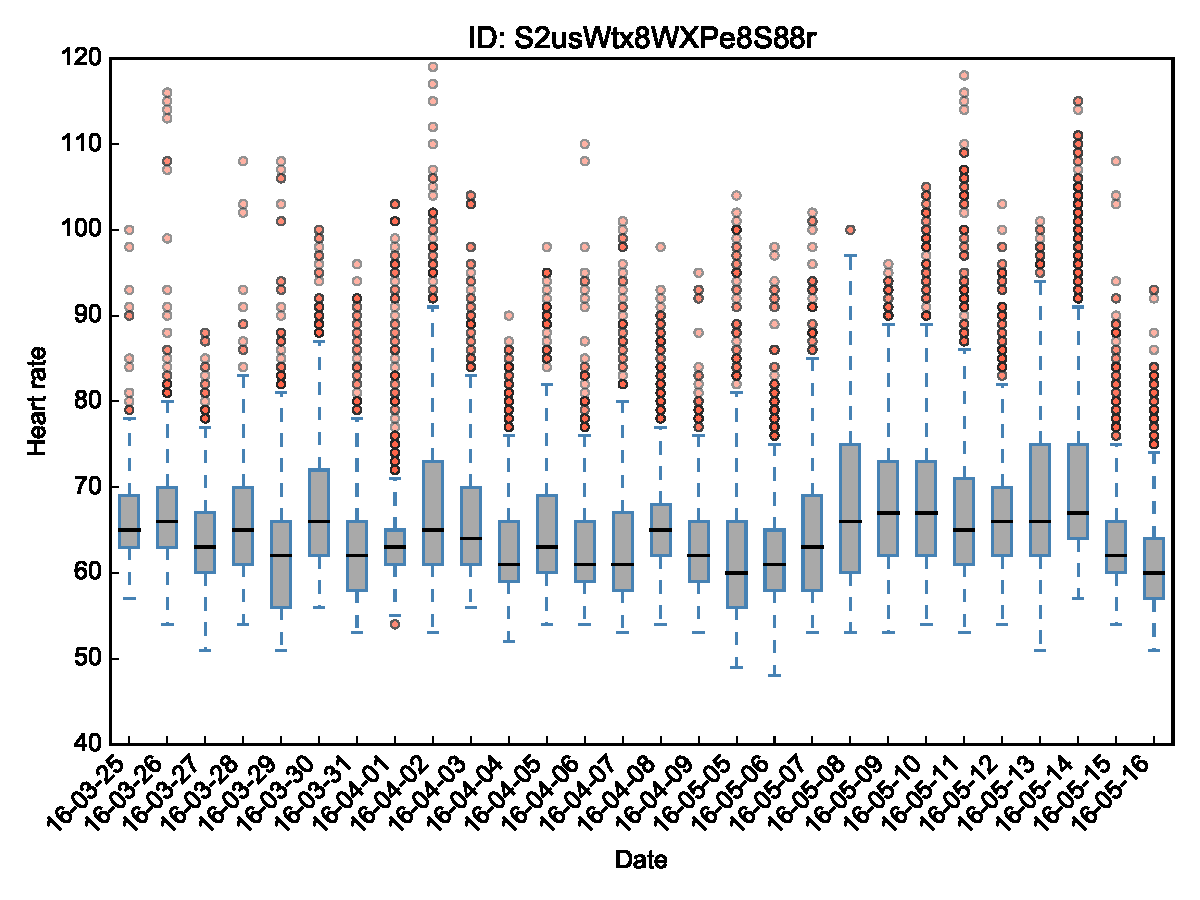
\includegraphics[scale=0.5]{boxplots/S2usWtx8WXPe8S88r}
	}
	\captionof{figure}{}
\end{figure}

\newpage

\section{Elliptic Outlier Detection}
%
\begin{code}
	\begin{minted}[linenos=true, fontsize=\footnotesize, breaklines=true]{python}
def PlotEllipticOutliers(rawPositions, ID, timestmp):
    """
    This method is used for outlier detection on a straight track.
    Uses the EllipticEnvelope object from Scikit-learn
    :param rawPositions:    The raw GPS positions
    :param ID:              The ID of the user
    :param timestmp:        The timestamp
    """
    folder = "out/"
    plotDir = folder + "plots/Walking Test"

    lats = []
    longs = []
    timestamps = []
    for pos in rawPositions:
        lat = pos["latitude"]
        long = pos["longitude"]
        timestamp = pos["timestamp"]
        lats.append(lat)
        longs.append(long)
        timestamps.append(timestamp)

    # writeToFile(ID, "output", lats, longs)
    classifiers = {
        "Robust Covariance Estimator": EllipticEnvelope(contamination=0.08, support_fraction=0.8)
    }
    alpha = 0.5
    linewidth = 0.15

    classifierName = "Robust Covariance Estimator"
    classifier = classifiers[classifierName]
    X = zip(lats, longs)
    xx1, yy1 = np.meshgrid(np.linspace(min(lats), max(lats), 1000), np.linspace(min(longs), max(longs), 1000))
    classifier.fit(X)
    Z1 = classifier.decision_function(np.c_[xx1.ravel(), yy1.ravel()])
    Z1 = Z1.reshape(xx1.shape)
    CS = plt.contour(xx1, yy1, Z1, levels=[0], linewidths=1, colors="g")
    CS.collections[0].set_label(classifierName)
    plt.scatter(lats, longs, s=50, alpha=alpha, linewidth=linewidth, edgecolor=almost_black, color="steelblue",
                label="GPS coordinate")
    plt.autoscale(enable=True, axis="both")
    filteredPositions = []

    for lat, long, timestamp in zip(lats, longs, timestamps):
        z = classifier.decision_function(np.c_[lat, long])
        if z > 0:  # Check if coordinate (lat, long) is within the ellipse
            filteredPositions.append((lat, long, timestamp))

    y = zip(*filteredPositions)[0]  # the latitudes
    x = zip(*filteredPositions)[1]  # the longitudes
    t = zip(*filteredPositions)[2]  # the timestamps

    x2, y2, newx2, newy2 = smooth(y, x, t)
    plt.plot(y2, x2, label="Linear Interpolation")
    totalDistance = calcDistanceWalked(newy2, newx2)

    plt.plot(newy2, newx2, label="Savgol Filter", color="r")
    plt.title("Timestamp: %s\n Calculated distance: %i meters" % (timestmp, totalDistance))
    plt.xlabel("Latitude")
    plt.ylabel("Longitude")
    fancyPlot()
    writeToPdf(ID, plotDir)

\end{minted}
	\caption{Code used for detecting outliers in a straight path.}
	\label{GPS Smoothing Code Straight Line}
\end{code}
%

\newpage

\section{Clustering Outlier Detection}
%
\begin{code}
	\begin{minted}[linenos=true, fontsize=\footnotesize, breaklines=true]{python}
def clustering(lats, longs, timestamps, ID, timestmp, multiPDF=False):
    """
    Clusters the GPS coordinates using DBSCAN
    :param timestmp:                The timestamp
    :param ID:                      The ID
    :param timestamps:              The timestamps of the GPS coordinates
    :param lats:                    The latitudes
    :param longs:                   The longitudes
    :return:                        The rounded distance
    """
    folder = "out/"
    plotDir = folder + "plots/Walking Test Analysis"

    R = 6371  # Radius of the earth in km
    cartesianX = []
    cartesianY = []
    cartesianZ = []

    for lat, long in zip(lats, longs):
        # Convert to cartesian coordinates
        x = R * cos(lat) * cos(long)
        y = R * cos(lat) * sin(long)
        z = R * sin(lat)
        cartesianX.append(x)
        cartesianY.append(y)
        cartesianZ.append(z)

    combined = np.vstack((cartesianX, cartesianY, cartesianZ)).T
    (core_samples, labels) = dbscan(combined, eps=0.5)
    grouped = zip(labels, core_samples)
    nonGroupedPositions = []

    for (label, core_sample) in grouped:
        if label != -1:
            lat = lats[core_sample]
            long = longs[core_sample]
            stamp = timestamps[core_sample]
            nonGroupedPositions.append((lat, long, stamp))

    if len(nonGroupedPositions) > 0:
        y = zip(*nonGroupedPositions)[0]  # the latitudes
        x = zip(*nonGroupedPositions)[1]  # the longitudes
        t = zip(*nonGroupedPositions)[2]  # the timestamps
        x2, y2, newx2, newy2 = smooth(y, x, t)

        plt.plot(y2, x2, label="Linear Interpolation")
        plt.plot(newy2, newx2, label="Savgol Filter", color="r")
        distance = calcDistanceWalked(newy2, newx2)
        grouped = sorted(grouped, key=itemgetter(0))

        clusters = {}
        labels = []
        for key, group in groupby(grouped, key=itemgetter(0)):
            # group the clusters based on their label
            labels.append(key)
            clusters[key] = [el[1] for el in group]

        noise = False
        colors = plt.get_cmap("Spectral")(np.linspace(0, 1, len(clusters)))
        for label in labels:
            indices = clusters[label]
            latitudes = []
            longitudes = []
            size = 10
            alpha = 0.5
            lineWidth = 0.15
            for i in indices:
                latitudes.append(lats[i])
                longitudes.append(longs[i])
            if label == -1:
                # outliers are identified with a label of -1
                plt.plot(latitudes, longitudes, "o", markerfacecolor=almost_black, markeredgecolor=almost_black,
                         markersize=size, alpha=alpha, linewidth=lineWidth, label="Outlier")
                noise = True
            else:
                plt.plot(latitudes, longitudes, "o", markerfacecolor=colors[label], markeredgecolor=almost_black,
                         markersize=size, alpha=alpha, linewidth=lineWidth, label="Cluster %i" % (label + 1))

        plt.title("Timestamp: %s\n Number of clusters: %i\n Calculated distance: %i meters" % (
            timestmp, (len(clusters) - 1) if noise else len(clusters), round(distance)))
        plt.xlabel("Latitude")
        plt.ylabel("Longitude")
        fancyPlot()
        writeToPdf(ID, plotDir)
        return True, distance
    else:
        # DBSCAN gave back an empty array, therefore we cannot perform any smoothing or distance calculation
        return False, 0
\end{minted}
	\caption{Code used for detecting outliers in a non-straight path.}
	\label{GPS Smoothing Code Non-Straight Line}
\end{code}
%

\newpage

\section{Calculation of Walking Speed}
%
\begin{code}
	\input{code/"Walking speed".tex}
	\caption{Code used for calculating the walking speed between GPS coordinates.}
	\label{walk test code snippet}
\end{code}
%


\section{Tables}
\subsection{Sleep}
% !TeX spellcheck = en_US
% !TeX root = ../BachelorThesis.tex

\begin{table}[H]
 	\centering
 	\begingroup
 	\fontsize{6pt}{6pt}
 	\selectfont
 	\subfloat[]{
 		\csvautobooktabular[head to column names, table head=\toprule \bfseries Date & \bfseries Rating & \bfseries Duration (h)\\\midrule]
 		{csv/sleep/2Dy2uFf3aw6jv9r5u.csv}
 		\label{table:sleepduration1}
 	}
 	\hspace{1cm}
 	\subfloat[]{
 		\csvautobooktabular[head to column names, table head=\toprule \bfseries Date & \bfseries Rating & \bfseries Duration (h)\\\midrule]
 		{csv/sleep/dW4YzJQEaidmyhsuY.csv}
 		\label{table:sleepduration2}
 	}
 	\captionof{table}{Measurements of the sleep duration of our participants.} 
	\label{table: Sleep Analysis}
	
	\endgroup
\end{table}

\begin{table}[H]
	\ContinuedFloat
	\centering
 	\begingroup
 	\fontsize{6pt}{6pt}
 	\selectfont
 	\subfloat[]{
 		\csvautobooktabular[head to column names, table head=\toprule \bfseries Date & \bfseries Rating & \bfseries Duration (h)\\\midrule]
 		{csv/sleep/gGSWzh5PnqgFdCpq4.csv}
 		\label{table:sleepduration3}
 	}
 	\hspace{1cm}
 	\subfloat[]{
 		\csvautobooktabular[head to column names, table head=\toprule \bfseries Date & \bfseries Rating & \bfseries Duration (h)\\\midrule]
 		{csv/sleep/S2usWtx8WXPe8S88r.csv}
 		\label{table:sleepduration4}
 	}
 	\captionof{table}{}
	\endgroup
\end{table}
\subsection{Heart Rate}
\input{tables/"heart rate"}
\subsection{Walking Test}
\input{tables/"walking test"}



\end{document}